\documentclass[conference]{IEEEtran}
\IEEEoverridecommandlockouts
\usepackage{cite}
\usepackage{amsmath,amssymb,amsfonts}
\usepackage{algorithmic}
\usepackage{graphicx}
\usepackage{textcomp}
\usepackage{xcolor}
\usepackage{url}
\def\BibTeX{{\rm B\kern-.05em{\sc i\kern-.025em b}\kern-.08em
    T\kern-.1667em\lower.7ex\hbox{E}\kern-.125emX}}
\begin{document}

\title{StoikovKV: Heterogeneous KV-Cache Compression with Query-Aware Routing and Self-Speculative Decoding}

\author{\IEEEauthorblockN{1\textsuperscript{st} Sai Rishi Gangarapu}
\IEEEauthorblockA{\textit{Department of Computer Science and Engineering} \\
\textit{PES University}\\
Bengaluru, India \\
sairishigangarapu@gmail.com}
\and
\IEEEauthorblockN{2\textsuperscript{nd} Ponakala Yathish}
\IEEEauthorblockA{\textit{Department of Computer Science and Engineering} \\
\textit{PES University}\\
Bengaluru, India \\
ponkalayathish@gmail.com}
\and
\IEEEauthorblockN{3\textsuperscript{rd} Pratham S Reddy}
\IEEEauthorblockA{\textit{Department of Computer Science and Engineering} \\
\textit{PES University}\\
Bengaluru, India \\
reddyprathams@gmail.com}
}

\maketitle

\begin{abstract}
Key-Value (KV) cache memory footprint and high-bandwidth memory (HBM) traffic are primary bottlenecks in long-context and multi-batch large language model (LLM) inference. Existing training-free compression schemes apply a uniform policy to every attention head, forcing an unfavorable tradeoff: heavy-hitter eviction methods struggle with early-context needle retention and stale multi-turn tokens, uniform low-bit quantization degrades sharp copy heads, and universal sparse dictionary coding incurs iterative solver overhead while distorting exact retrieval. Guided by the principle that distinct attention heads exhibit sharply different information-retention requirements, we present \textbf{StoikovKV}, a heterogeneous per-KV-head compression and self-speculative decoding engine for Grouped-Query Attention (GQA) transformers. During one-time offline calibration using projection hooks and streaming $64$-query chunked statistics, StoikovKV extracts a sign-aligned low-rank query subspace $U_Q$ per KV-head group, partitions heads into three tiers (exact FP16 retrieval heads, compacted heavy-hitter eviction heads, and sparse dictionary heads), and computes a double-precision ridge preconditioner $W_{\text{ridge}}$ in the pre-rotary embedding frame. During online inference---which executes with \texttt{output\_attentions=False} and zero quadratic attention materialization---StoikovKV scores incoming tokens at write time via directional query-subspace probing and pre-RoPE key rarity spans, refreshes stale heavy hitters upon topic transitions via an online regime-change decay controller, and compresses diffuse heads with One-Step Ridge-Preconditioned Thresholded Sparse Coding into descending-magnitude atoms. Reading a truncated atom prefix enables single-model Matryoshka self-speculative drafting with strict lossless rejection-sampling verification. Evaluated on real pretrained \texttt{Qwen/Qwen2.5-1.5B-Instruct}, \texttt{Qwen/Qwen2.5-3B-Instruct}, and offloaded \texttt{Qwen/Qwen2.5-7B-Instruct} checkpoints using unseen passkeys planted in external Paul Graham essays at a $\sim 21\%$ KV budget, StoikovKV achieves $85.0\%$ ($17/20$, $95\%$ CI $[64.0\%, 94.8\%]$) on 1.5B, $100.0\%$ ($16/16$, $95\%$ CI $[80.6\%, 100.0\%]$) on 3B, and $100.0\%$ ($8/8$, $95\%$ CI $[67.6\%, 100.0\%]$) on 7B with consistently higher next-token logit fidelity ($0.8855$--$0.9371$) than SnapKV and H2O, while delivering $5.78\times$--$37.58\times$ faster encoding than OMP on $1{,}024$ distinct real KV vectors, $32/32$ bit-exact greedy speculative parity, and $2.11\times$ higher maximum aggregate throughput under a fixed $128\text{ MB}$ KV-pool ceiling.
\end{abstract}

\begin{IEEEkeywords}
large language models, key-value cache compression, grouped-query attention, heterogeneous head routing, query subspace probing, sparse dictionary coding, speculative decoding
\end{IEEEkeywords}

\section{Introduction}
Autoregressive decoding in large language models (LLMs) is fundamentally memory-bandwidth bound. Even with Grouped-Query Attention (GQA) \cite{b1}, which shares each Key-Value (KV) head across $g = H_Q / H_{KV}$ query heads, long-context multi-turn conversations, retrieval-augmented generation (RAG), and high-concurrency batch serving rapidly exhaust GPU High-Bandwidth Memory (HBM). At every decoding step, the entire resident KV cache must be streamed from HBM into on-chip SRAM, throttling arithmetic utilization and capping the maximum feasible serving batch size.

The central research proposition of this work is straightforward: \emph{different attention heads have fundamentally different information-retention requirements, so KV-cache compression should be heterogeneous rather than uniform.} Mechanistic interpretability studies confirm that fewer than $\sim 5\%$ of attention heads act as exact long-range retrieval/copy heads \cite{b14}, whereas the majority concentrate attention locally on syntax or heavy hitters, and a remaining high-entropy subset integrates information diffusely across the entire sequence. Enforcing a single homogeneous compression strategy across all heads creates three failure modes:
\begin{enumerate}
    \item \textbf{Early-Needle Blindness and FlashAttention Constraints in Token Eviction:} Heavy-Hitter Oracle (H2O) \cite{b2} and StreamingLLM \cite{b3} evict low-scoring tokens globally, but standard H2O relies on explicit $O(T^2)$ attention matrices that fused kernels such as FlashAttention-2 \cite{b4} and PyTorch SDPA never materialize during inference. Moreover, when an early fact is queried thousands of tokens later, intermediate filler crowds it out, and local suffix-window methods such as SnapKV \cite{b5} fail whenever an abrupt topic shift separates the needle from the observation window.
    \item \textbf{Multi-Turn Cache Stagnation:} Under cumulative importance scoring, tokens from an earlier conversation turn accumulate large scores that persist after a topic transition, preventing heavy-hitter slots from adapting to the active turn.
    \item \textbf{Copy-Head Blurring and Solver Latency in Uniform Quantization and Sparse Coding:} Uniform $2$-bit quantization (e.g., KIVI \cite{b6}) and universal sparse dictionary coding (e.g., Lexico \cite{b7}) retain all $T$ sequence positions across every head. Compressing sharp retrieval heads with coarse quantization or $s$-sparse approximations degrades exact passkey logits, while iterative sparse solvers such as Orthogonal Matching Pursuit (OMP) or FISTA \cite{b8} introduce millisecond-scale encoding stalls and struggle with position-dependent Rotary Position Embeddings (RoPE) \cite{b9}.
\end{enumerate}

To resolve these tradeoffs, we introduce \textbf{StoikovKV}, a unified KV-cache compression and self-speculative decoding system for GQA transformers. Our main contributions are:
\begin{itemize}
    \item \textbf{FlashAttention-Compatible Online Write-Time Subspace Probing:} Using a one-time offline streaming hook profiler, we extract a sign-aligned rank-$r$ ($r = 16$) query subspace $U_Q \in \mathbb{R}^{d \times r}$ per KV head. At inference time (\texttt{output\_attentions=False}), incoming tokens are scored in $O(d \cdot r)$ operations without materializing $T \times T$ attention matrices, outperforming the value-norm baseline $\|V_t\|_2$ by $+0.4795$ to $+0.6087$ Spearman $\rho$ across real \texttt{Qwen2.5-1.5B}, \texttt{3B}, and \texttt{7B} checkpoints.
    \item \textbf{Three-Tier Per-KV-Head Routing with Layer Co-Location and Online Regime-Change Decay:} StoikovKV assigns KV heads to uncompressed FP16 retrieval ($\sim 5.4\%$), physically compacted heavy-hitter eviction ($\sim 89\%$), and pre-RoPE sparse dictionary coding ($\sim 5.4\%$). Co-locating diffuse and retrieval heads leaves $\sim 89\%$ of layers pure H2O with a virtual partition sink, while an online EMA regime-change detector accelerates heavy-hitter decay ($\beta_{\text{shift}} = 0.65$ vs. $\beta_{\text{stat}} = 0.99$) across topic transitions.
    \item \textbf{One-Step Ridge-Preconditioned Thresholded Sparse Coding:} Using an offline FP64 ridge preconditioner $W_{\text{ridge}}$ trained in the pre-RoPE frame, live encoding requires a single GEMM, soft-thresholding, descending-magnitude top-$s$ selection, and scalar rescaling ($3s + 2$ bytes/vector), running $5.78\times$--$37.58\times$ faster than OMP on $1{,}024$ strictly distinct real KV vectors while staying within $0.006$--$0.010$ cosine similarity.
    \item \textbf{Audited Single-Model Matryoshka Self-Speculative Decoding:} Descending-magnitude atom ordering produces nested prefix approximations ($m < s$) that enable single-model drafting with strict lossless rejection sampling (\texttt{strict\_rejection\_sampling=True}), verified at $32/32$ ($100.0\%$) bit-exact greedy token parity on real \texttt{Qwen2.5-1.5B-Instruct}.
\end{itemize}

\section{Related Work}
\textbf{Token Eviction and Attention Sinks.} StreamingLLM \cite{b3} showed that preserving initial sink tokens alongside a local sliding window stabilizes infinite-length generation, while H2O \cite{b2} retains high cumulative-attention heavy hitters. SnapKV \cite{b5} pools attention within a suffix observation window to select important prompt positions before decoding. Unlike these homogeneous methods, StoikovKV separates eviction from retrieval-critical heads, computes online token importance without materializing attention matrices, and adds topic-shift-aware decay plus pre-RoPE rarity span protection.

\textbf{Mechanistic Retrieval Heads.} Wu et al.~\cite{b14} demonstrated that a sparse, intrinsic subset of attention heads ($<5\%$) mechanistically governs long-context factuality and Needle-in-a-Haystack copy behavior, and that pruning or corrupting these heads triggers hallucination. StoikovKV operationalizes this insight directly inside a live GQA cache by locking the top $5\%$ needle-selective KV heads in uncompressed FP16 while compressing the remaining $\sim 95\%$.

\textbf{Low-Bit Quantization and Sparse Dictionary Coding.} KIVI \cite{b6} applies tuning-free $2$-bit asymmetric quantization per-channel for keys and per-token for values. Lexico \cite{b7} compresses KV states via sparse linear combinations over a universal dictionary using iterative OMP. StoikovKV avoids compressing retrieval heads altogether, un-rotates keys to the pre-RoPE frame before dictionary coding, and replaces iterative OMP with a non-iterative one-step FP64 ridge-preconditioned thresholded encoder.

\textbf{Speculative Decoding and Nested Representations.} Leviathan et al.~\cite{b12} introduced lossless speculative decoding using a separate draft model and rejection sampling to preserve the exact target distribution. Matryoshka Representation Learning \cite{b10} demonstrated nested multi-granularity embeddings. StoikovKV combines these ideas inside a single checkpoint and cache by drafting from truncated magnitude-sorted atom prefixes ($m \ll s$) and verifying in one batched pass at full sparsity $s$.

\section{Design Overview}
\begin{figure*}[t]
\centerline{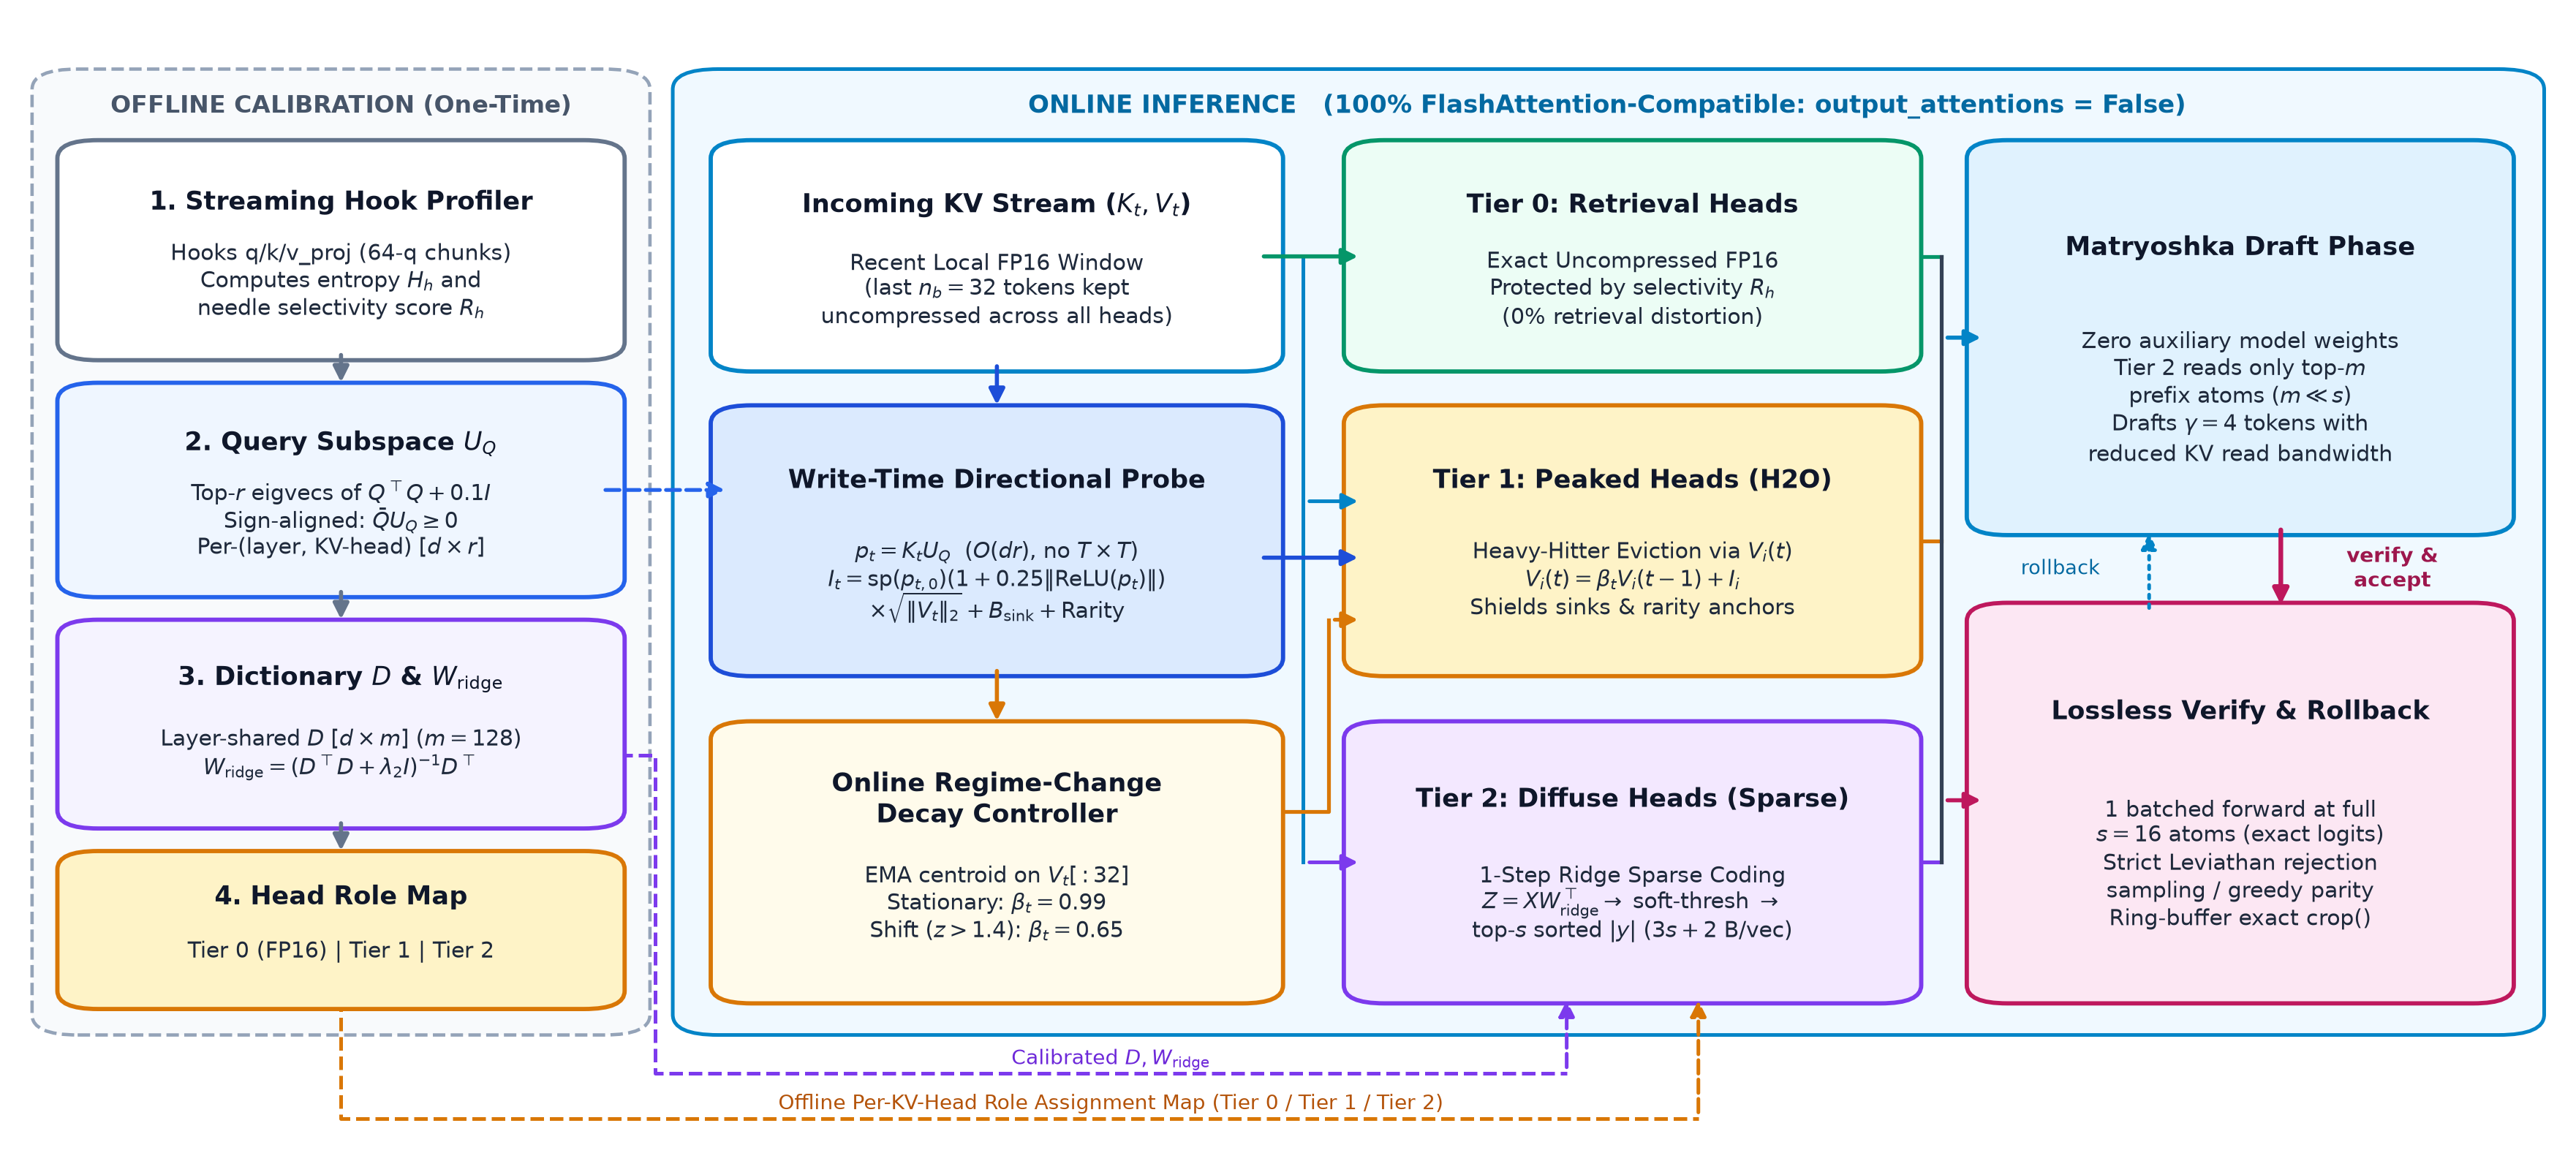
\includegraphics[width=\textwidth]{architecture_diagram.png}}
\caption{End-to-end StoikovKV architecture. One-time offline calibration extracts sign-aligned query subspaces $U_Q$, layer-shared pre-RoPE dictionaries $(D, W_{\text{ridge}})$, and per-KV-head tier assignments via streaming projection hooks. Online inference runs with \texttt{output\_attentions=False}, combining write-time directional probing, online regime-change decay, three-tier per-head storage, and single-model Matryoshka self-speculative verification.}
\label{fig:arch}
\end{figure*}

Fig.~\ref{fig:arch} illustrates the complete StoikovKV architecture split cleanly into two phases: a one-time offline calibration stage and a FlashAttention-compatible online inference engine.

\subsection{Conceptual Motivation from Inventory Control}
The architecture's three-tier routing and adaptive decay heuristics are conceptually motivated by the Avellaneda--Stoikov market-making inventory-control equations \cite{b13}. For an agent holding signed inventory $q$ under mid-price $s$, volatility $\sigma$, risk aversion $\gamma_{\text{risk}}$, order intensity $\kappa$, and remaining horizon $(T - t)$, the reservation price $r(s, q, t)$ and optimal spread $\delta_a + \delta_b$ satisfy:
\begin{equation}
r(s, q, t) = s - q \gamma_{\text{risk}} \sigma^2 (T - t),
\label{eq:as_reservation}
\end{equation}
\begin{equation}
\delta_a + \delta_b = \gamma_{\text{risk}} \sigma^2 (T - t) + \frac{2}{\gamma_{\text{risk}}} \ln\!\left(1 + \frac{\gamma_{\text{risk}}}{\kappa}\right).
\label{eq:as_spread}
\end{equation}
We emphasize that \eqref{eq:as_reservation}--\eqref{eq:as_spread} serve strictly as a conceptual design analogy rather than a formal Hamilton--Jacobi--Bellman optimality proof for KV caches. Specifically, the analogy motivates four concrete engineering choices that stand independently on empirical performance: (1) estimating token utility $I_t$ at write time (analogous to mid-price $s$); (2) enforcing a fixed memory cap via eviction or sparse coding when cache occupancy grows (inventory pressure $q$); (3) accelerating stale heavy-hitter decay when online feature drift spikes (volatility $\sigma^2$); and (4) routing heads by their eviction sensitivity (risk aversion $\gamma_{\text{risk}}$) into exact FP16, heavy-hitter eviction, or sparse dictionary tiers.

\subsection{End-to-End Online Dataflow}
Every layer maintains an uncompressed recent sliding window of $n_b = 32$ tokens across all KV heads so local syntactic dependencies remain exact. As tokens age out of this window, each KV head $(l, h)$ routes them strictly according to its offline-assigned role into either Tier 0 (exact FP16), Tier 1 (physically compacted heavy-hitter buffer), or Tier 2 (pre-RoPE sparse dictionary payload). Importantly, \texttt{StoikovKVCache} inherits from HuggingFace \texttt{DynamicCache} without duplicating tensors in \texttt{key\_cache}/\texttt{value\_cache}, ensuring that logical compressed KV bytes equal physical resident GPU tensor bytes (\texttt{compressed\_bytes == physical\_resident\_bytes}).

\section{Query-Aware Calibration and Routing}

\subsection{FlashAttention Compatibility Scope}
Because prior KV-cache literature frequently conflates calibration and inference requirements, we state the exact attention-materialization boundary of StoikovKV:
\begin{itemize}
    \item \textbf{Online Inference (100\% FlashAttention/SDPA-Compatible):} Live prefill, autoregressive decoding, write-time probing, regime-change detection, three-tier routing, and Matryoshka speculative decoding run strictly with \texttt{output\_attentions=False}. No $T \times T$ attention matrix is ever materialized.
    \item \textbf{Offline Calibration (One-Time Streaming Hooks):} Measuring per-head causal entropy $H_{l,h}$ and needle selectivity $R_{l,h}$ requires attention statistics. Rather than running quadratic eager attention during the model forward pass, \texttt{calibrate\_model} registers forward hooks on \texttt{q\_proj}, \texttt{k\_proj}, and \texttt{v\_proj} while executing standard SDPA (\texttt{output\_attentions=False}), then computes exact causal entropy and column-wise attention sums in streaming $64$-query chunks ($O(B \cdot T)$ peak memory). Legacy unit-test fallbacks retain an optional \texttt{output\_attentions=True} path for standalone harnesses, which is never used in live inference.
\end{itemize}

\subsection{Sign-Aligned Query Subspace Extraction}
For a GQA transformer with $L$ layers, $H_Q$ query heads, $H_{KV}$ KV heads ($g = H_Q / H_{KV}$), and head dimension $d = 128$, let $Q_{l,h} \in \mathbb{R}^{M \times d}$ denote the post-RoPE query states pooled across all $g$ query heads sharing KV head $h$ over the calibration prompts ($N_{\text{cal}} = 16$ on 1.5B/3B; $N_{\text{cal}} = 8$ on 7B). In exact correspondence with \texttt{calibration.py}, we compute the regularized uncentered second-moment matrix in FP32 on CPU:
\begin{equation}
\Sigma_{l,h} = Q_{l,h}^\top Q_{l,h} + 0.1 \, I_d,
\label{eq:uncentered_cov}
\end{equation}
and extract its top-$r$ ($r = 16$) orthonormal eigenvectors $V_{l,h} = [v_0, \dots, v_{r-1}] \in \mathbb{R}^{d \times r}$ sorted in descending eigenvalue order via \texttt{torch.linalg.eigh} (with an SVD fallback if needed). Because eigenvectors are unique only up to sign while exponential softmax attention $\exp(q \cdot k / \sqrt{d})$ is strongly sign-sensitive, we align every basis column against the empirical mean query $\bar{q}_{l,h} = \frac{1}{M}\sum_{i=1}^M Q_{l,h,i}$:
\begin{equation}
u_k = \text{sign}^{*}\!\left(\bar{q}_{l,h}^\top v_k\right) v_k, \quad \text{sign}^{*}(x) = \begin{cases} -1, & x < 0, \\ +1, & x \ge 0, \end{cases}
\label{eq:sign_align}
\end{equation}
yielding $U_{Q,l,h} = [u_0, \dots, u_{r-1}] \in \mathbb{R}^{d \times r}$ with $U_{Q,l,h}^\top U_{Q,l,h} = I_r$ and $\bar{q}_{l,h}^\top U_{Q,l,h} \ge \mathbf{0}$.

\subsection{Write-Time Directional Probe and Pre-RoPE Rarity Spans}
At write time, for an incoming post-RoPE key $K_t \in \mathbb{R}^d$ and value $V_t \in \mathbb{R}^d$, we compute the low-rank projection $p_t = K_t U_{Q,l,h} \in \mathbb{R}^r$ in $O(d \cdot r)$ operations. To match \texttt{score\_write\_time} in \texttt{calibration.py} and \texttt{cache.py} verbatim, the write-time salience score is:
\begin{equation}
\begin{aligned}
I_t^{\text{HF}} = {} & \text{softplus}(p_{t,0})\!\left(1 + 0.25\|\text{ReLU}(p_t)\|_2\right)\sqrt{\|V_t\|_2} \\
                     & + B_{\text{sink}}\mathbb{I}[t < 4],
\end{aligned}
\label{eq:write_probe_hf}
\end{equation}
on pretrained HuggingFace checkpoints (where mean value norms exceed $4.0$ and $\sqrt{\|V_t\|_2}$ damps heavy-tailed norm variance), and at unit activation scale (standalone GQA harnesses):
\begin{equation}
I_t^{\text{unit}} = \sigma(p_{t,0}) \cdot \|p_t\|_2 \cdot \|V_t\|_2 + B_{\text{sink}}\mathbb{I}[t < 4],
\label{eq:write_probe_unit}
\end{equation}
with $B_{\text{sink}} = 100.0$ preserving the initial $T_{\text{sink}} = 4$ attention sinks \cite{b3}. Note that unlike an unsigned projection norm $\|K_t U_Q\|_2 \|V_t\|_2$, gating by $\text{softplus}(p_{t,0})$ suppresses keys anti-aligned with $\bar{q}_{l,h}$.

During hybrid prefill ($q_{\text{len}} \ge 64$) on pretrained models, multi-digit passkeys split across $5$ BPE tokens and risk partial eviction when surrounded by long prose. Un-rotating keys into the position-free pre-RoPE frame $\hat{K}_{\text{pre}, t} = R_{-\theta, t} K_t / \|K_t\|_2$ exposes repeated background phrases via high distant cosine similarity ($|t - t'| > 40$), whereas unique factual spans exhibit high distant rarity:
\begin{equation}
\begin{aligned}
\mathcal{R}_{\text{span}}(t) = \text{AvgPool}_{w=15}\Biggl(1 - \frac{1}{k}\sum_{j=1}^{k} & \text{TopK}_{|t-t'|>40} \\
& \Bigl(\langle \hat{K}_{\text{pre},t}, \hat{K}_{\text{pre},t'}\rangle\Bigr)_j\Biggr).
\end{aligned}
\label{eq:rarity_span}
\end{equation}
The top $4.5\%$ rarity-span tokens receive an anchor boost ($+80.0 + 8.0\,\mathcal{R}_{\text{span}}(t)$), keeping multi-token entities contiguous across eviction boundaries.

\subsection{Three-Tier Head Classification and Calibration Separation}
From the streaming hook statistics over the calibration prompts plus $4$ synthetic needle prompts containing calibration code \texttt{"94812"} (strictly disjoint from all held-out evaluation prompts and all external Paul Graham essay passkeys), we compute distractor-adjusted needle selectivity $R_{l,h} = \max(0, \bar{A}_{\text{needle},l,h} - 0.5\bar{A}_{\text{distractor},l,h})$ and mean causal entropy $H_{l,h}$. The top $5\%$ of KV heads by $R_{l,h}$ ($3/56$ on 1.5B, $4/72$ on 3B, $6/112$ on 7B) are locked in \textbf{Tier 0 (\texttt{ROLE\_RETRIEVAL\_FP16})}. Among remaining heads, those below the 90th-percentile entropy threshold become \textbf{Tier 1 (\texttt{ROLE\_PEAKED\_H2O})}, while the highest-entropy heads become \textbf{Tier 2 (\texttt{ROLE\_DIFFUSE\_LEXICO})}, co-located onto the same layers as Tier 0 so that $25/28$ layers ($89.3\%$) on 1.5B and 7B ($32/36$, $88.9\%$ on 3B) are layer-pure Tier 1.

In layer-pure Tier-1 layers, evicted history keys ($n_{\text{evict}} = T_{\text{hist}} - k_{\text{kept}}$) are physically removed rather than masked, and a single \textbf{virtual partition sink} token is prepended:
\begin{equation}
k_{\text{sink}} = \alpha_{\text{sink}}\ln(n_{\text{evict}})\,u_0, \quad v_{\text{sink}} = \mathbf{0} \in \mathbb{R}^d,
\label{eq:virtual_sink}
\end{equation}
approximating the missing softmax partition mass without inflating physical sequence length beyond $k_{\text{kept}} + 1 + n_b \ll T$.

\section{Hybrid KV Compression}

\subsection{Online Regime-Change Decay Controller}
To prevent Turn-1 heavy hitters from monopolizing Tier-1 slots after a multi-turn topic transition, StoikovKV runs an \textbf{Online Regime-Change Decay Controller} (implemented as \texttt{HMMTopicShiftController} in \texttt{cache.py}). We clarify that this controller is an online Exponential Moving Average (EMA) centroid/deviation regime detector rather than a probabilistic Hidden Markov Model with Viterbi or Baum--Welch inference. Over $64$-token chunks on layer $0$, it forms a unit-normalized position-free value feature $f_c = \text{normalize}(\bar{V}_{c, :32})$, tracks EMA centroid $\mu_c$ and deviation $\sigma_c$ ($\alpha_{\text{EMA}} = 0.15$), and evaluates normalized drift $z_c = \|f_c - \mu_c\|_2 / \max(\sigma_c, 10^{-4})$. Whenever $z_c > \tau_z = 1.4$, the controller pulses the decay factor from $\beta_{\text{stat}} = 0.99$ to $\beta_{\text{shift}} = 0.65$:
\begin{equation}
S_i(t) = \begin{cases}
S_i(t-1) + I_i, & S_i \ge 60\text{ (anchor)}, \\
\beta_t^{\Delta t / 16} S_i(t-1) + I_i, & \text{otherwise},
\end{cases}
\label{eq:regime_decay}
\end{equation}
flushing stale background heavy hitters while shielding attention sinks and high-rarity anchors.

\subsection{One-Step Ridge-Preconditioned Thresholded Sparse Coding}
For Tier-2 (\texttt{ROLE\_DIFFUSE\_LEXICO}) heads, keys are first un-rotated into the position-free pre-RoPE frame ($K_{\text{pre},t} = R_{-\theta,t} K_t$) so a single static dictionary $D_l \in \mathbb{R}^{d \times N}$ ($N = 128$, unit-norm columns) represents keys across arbitrary sequence positions; RoPE is re-applied upon decoding. Offline, we refine $D_l$ on calibration KV vectors and solve the ridge preconditioner in \textbf{FP64}:
\begin{equation}
W_{\text{ridge}, l} = \left(D_l^\top D_l + \lambda_2 I_N\right)^{-1} D_l^\top, \quad \lambda_2 = 0.1,
\label{eq:w_ridge}
\end{equation}
achieving linear-solve relative residuals $< 7.5 \times 10^{-16}$ across all evaluated checkpoints.

At inference time, rather than solving the iterative ElasticNet objective to convergence, we apply \textbf{One-Step Ridge-Preconditioned Thresholded Sparse Coding} as a fast single-pass approximation. Given $\tilde{x} = (N / d)\cdot x / \|x\|_2$:
\begin{equation}
z = W_{\text{ridge}, l}\tilde{x}, \quad y = \text{sign}(z) \odot \max\!\left(0, |z| - \lambda_1\right).
\label{eq:one_step_codec}
\end{equation}
We select the top-$s$ entries of $|y|$ sorted in descending magnitude order $|y_{(1)}| \ge |y_{(2)}| \ge \dots \ge |y_{(s)}|$ with support $\mathcal{I}_s$, apply scalar norm-matching rescaling $\hat{y}_s = y_s \cdot (\|x\|_2 / \|D_{l,\mathcal{I}_s} y_s\|_2)$, and quantize $\hat{y}_s$ to \texttt{int8} with an FP16 scale. The resulting payload is exactly $3s + 2$ bytes/vector ($2s$ bytes \texttt{int16} indices, $s$ bytes \texttt{int8} coefficients, $2$ bytes FP16 scale) versus $256$ bytes in FP16 ($5.12\times$ payload compression at $s = 16$). Because $D_l$ and $W_{\text{ridge},l}$ reside once per active Tier-2 layer ($64\text{ KB}$ total per layer in FP16), they amortize once the layer stores $L^* = B_{\text{dict}} / (256 - (3s + 2))$ vectors ($L^* \approx 318$ vectors at $s = 16$). Throughout our evaluation, we report both compressed KV payload bytes (\texttt{KV Mem \%}) and total resident bytes including dictionaries (\texttt{+Dict \%}).

\section{Matryoshka Self-Speculative Decoding}
Because every Tier-2 vector stores its $s$ sparse coefficients in descending magnitude order $|y_{(1)}| \ge \dots \ge |y_{(s)}|$, slicing the first $m < s$ entries yields a nested prefix approximation \cite{b10} with zero duplicate storage or re-encoding. We note carefully that magnitude-sorted prefixes provide a convenient nested representation rather than a formal guarantee of globally MSE-optimal $m$-sparse reconstructions for every $m$.

During each self-speculative decoding cycle (\texttt{matryoshka\_speculative\_generate}):
\begin{enumerate}
    \item \textbf{Reduced-Bandwidth Draft Phase ($\gamma_{\text{spec}} = 4$):} Calling \texttt{cache.set\_matryoshka\_mode(active\_atoms=m)} ($m \in \{2, 4, 8, 12\}$) instructs Tier-2 heads to read only \texttt{indices[..., :m]} and \texttt{values[..., :m]} ($3m + 2$ B/vec) while Tier-0 and Tier-1 heads remain unchanged, drafting $\gamma_{\text{spec}}$ tokens $d_1, \dots, d_{\gamma_{\text{spec}}}$ with draft distributions $q_1, \dots, q_{\gamma_{\text{spec}}}$.
    \item \textbf{Single-Pass Batched Verification ($\gamma_{\text{spec}} + 1$ tokens):} Temporary draft KV states are rolled back via ring-buffer \texttt{cache.crop(L\_base)}, full verification sparsity \texttt{active\_atoms=s} ($s = 16$) is restored, and one batched forward pass evaluates $[t_{\text{last}}, d_1, \dots, d_{\gamma_{\text{spec}}}]$ to obtain target distributions $p_1, \dots, p_{\gamma_{\text{spec}}+1}$.
    \item \textbf{Audited Lossless Rejection Sampling:} To guarantee exact target-distribution equivalence \cite{b12}, \texttt{strict\_rejection\_sampling=True} is enabled by default in \texttt{matryoshka\_spec.py}, disabling all heuristic logit adjustments or token suppression so draft ($q_j$) and target ($p_j$) distributions share identical raw model logits, temperature, and top-$k$ vocabulary support. In greedy mode (\texttt{do\_sample=False}), draft token $d_j$ is accepted iff $d_j = \arg\max p_j$; in stochastic mode, $d_j$ is accepted with probability $\min(1, p_j(d_j)/q_j(d_j))$, with first rejection resampled from $\text{norm}(\max(0, p_j - q_j))$ and cache rolled back via \texttt{cache.crop(L\_base + j)}. Full acceptance emits the $(\gamma_{\text{spec}} + 1)$-th bonus token from $p_{\gamma_{\text{spec}}+1}$.
\end{enumerate}

\section{Experimental Evaluation}

\subsection{Experimental Setup, Models, and Datasets}
All experiments run locally on a single NVIDIA GeForce RTX 4060 Laptop GPU ($8\text{ GB}$ VRAM, CUDA 13.0, PyTorch \texttt{2.12.0+cu130}, \texttt{torch.float16}) with $15\text{ GB}$ host RAM. To rigorously distinguish real-model behavior from controlled ablations, we separate four evaluation tracks:
\begin{enumerate}
    \item \textbf{Multi-Scale External Paul Graham Essays NIAH (Primary Real-Model Track):} We evaluate real pretrained \texttt{Qwen/Qwen2.5-1.5B-Instruct} ($28$L, $12$Q/$2$KV, 100\% GPU FP16), \texttt{Qwen/Qwen2.5-3B-Instruct} ($36$L, $16$Q/$2$KV, 100\% GPU FP16), and \texttt{Qwen/Qwen2.5-7B-Instruct} ($28$L, $28$Q/$4$KV, exact FP16 split cleanly via \texttt{accelerate} across $7$ GPU / $5$ CPU / $16$ NVMe disk layers to prevent OOM under $8\text{ GB}$ VRAM and $15\text{ GB}$ RAM) \cite{b11}. Haystacks are drawn from the external Kamradt \texttt{LLMTest\_NeedleInAHaystack} corpus ($50$ Paul Graham essays, $8.3\text{ MB}$) \cite{b15}, with strictly unseen 5-digit passkeys (disjoint from calibration code \texttt{"94812"}) across $4$ depths $\{10\%, 25\%, 50\%, 75\%\}$. We report exact numerators, denominators, and $95\%$ Wilson confidence intervals.
    \item \textbf{Distinct Real-Prose Codec \& Strict Speculative Parity Track:} Evaluated on $1{,}024$ \emph{strictly distinct, non-tiled} KV vectors extracted from held-out Paul Graham essays on \texttt{Qwen2.5-1.5B}, plus strict lossless speculative parity (\texttt{strict\_rejection\_sampling=True}).
    \item \textbf{Multi-Turn Topic-Shift \& Memory-Ceiling Batch Scaling Track (\texttt{Qwen2.5-1.5B}):} Controlled $1{,}024$-token two-turn CSS shift ablation ($4$ needle depths) and $128\text{ MB}$ KV-pool batch scaling ($B \in \{1, 2, 4, 8, 12\}$).
    \item \textbf{Controlled Standalone GQA Ablation Track:} Synthetic $28$-layer GQA ($2{,}037$-token multi-turn, $135$-run multi-length NIAH up to $4{,}096$ tokens) and compact $12$-layer WikiText-103 \cite{b16} throughput ablation, clearly isolated from real-checkpoint metrics.
\end{enumerate}

\begin{table}[t]
\caption{Multi-Scale Held-Out Write-Time Directional Subspace Probe Correlation Across Real Pretrained \texttt{Qwen2.5} Checkpoints}
\begin{center}
\resizebox{\columnwidth}{!}{%
\begin{tabular}{|l|c|c|c|}
\hline
\textbf{Model / Probe Variant} & \textbf{Pairs} & \textbf{Spearman $\rho$} & \textbf{Recall@20\%} \\
\hline
\multicolumn{4}{|c|}{\textit{Real \texttt{Qwen/Qwen2.5-1.5B-Instruct} (100\% GPU FP16, Calib: $11.57\text{ s}$)}} \\
\hline
\textbf{Sink-Aug. Directional Probe} & 336 & \textbf{0.5733 $\pm$ 0.2716} & \textbf{52.19\% $\pm$ 18.09\%} \\
Raw Directional Probe ($t \ge 4$)    & 336 & 0.4020 $\pm$ 0.2887 & 36.73\% $\pm$ 18.67\% \\
Value-Norm Baseline ($\|V_t\|_2$)    & 336 & $-0.0354$ & 22.70\% \\
\hline
\multicolumn{4}{|c|}{\textit{Real \texttt{Qwen/Qwen2.5-3B-Instruct} (100\% GPU FP16, Calib: $15.59\text{ s}$)}} \\
\hline
\textbf{Sink-Aug. Directional Probe} & 432 & \textbf{0.5655 $\pm$ 0.2456} & \textbf{52.64\% $\pm$ 15.99\%} \\
Raw Directional Probe ($t \ge 4$)    & 432 & 0.3903 $\pm$ 0.2758 & 35.94\% $\pm$ 18.05\% \\
Value-Norm Baseline ($\|V_t\|_2$)    & 432 & $-0.0031$ & 23.11\% \\
\hline
\multicolumn{4}{|c|}{\textit{Real \texttt{Qwen/Qwen2.5-7B-Instruct} (GPU/CPU/NVMe FP16, Calib: $85.88\text{ s}$)}} \\
\hline
\textbf{Sink-Aug. Directional Probe} & 672 & \textbf{0.4838 $\pm$ 0.2908} & \textbf{49.72\% $\pm$ 16.55\%} \\
Raw Directional Probe ($t \ge 4$)    & 672 & 0.3491 $\pm$ 0.3413 & 37.10\% $\pm$ 21.28\% \\
Value-Norm Baseline ($\|V_t\|_2$)    & 672 & $+0.0043$ & 23.27\% \\
\hline
\end{tabular}%
}
\label{tab:probe_corr}
\end{center}
\end{table}

\begin{figure}[t]
\centerline{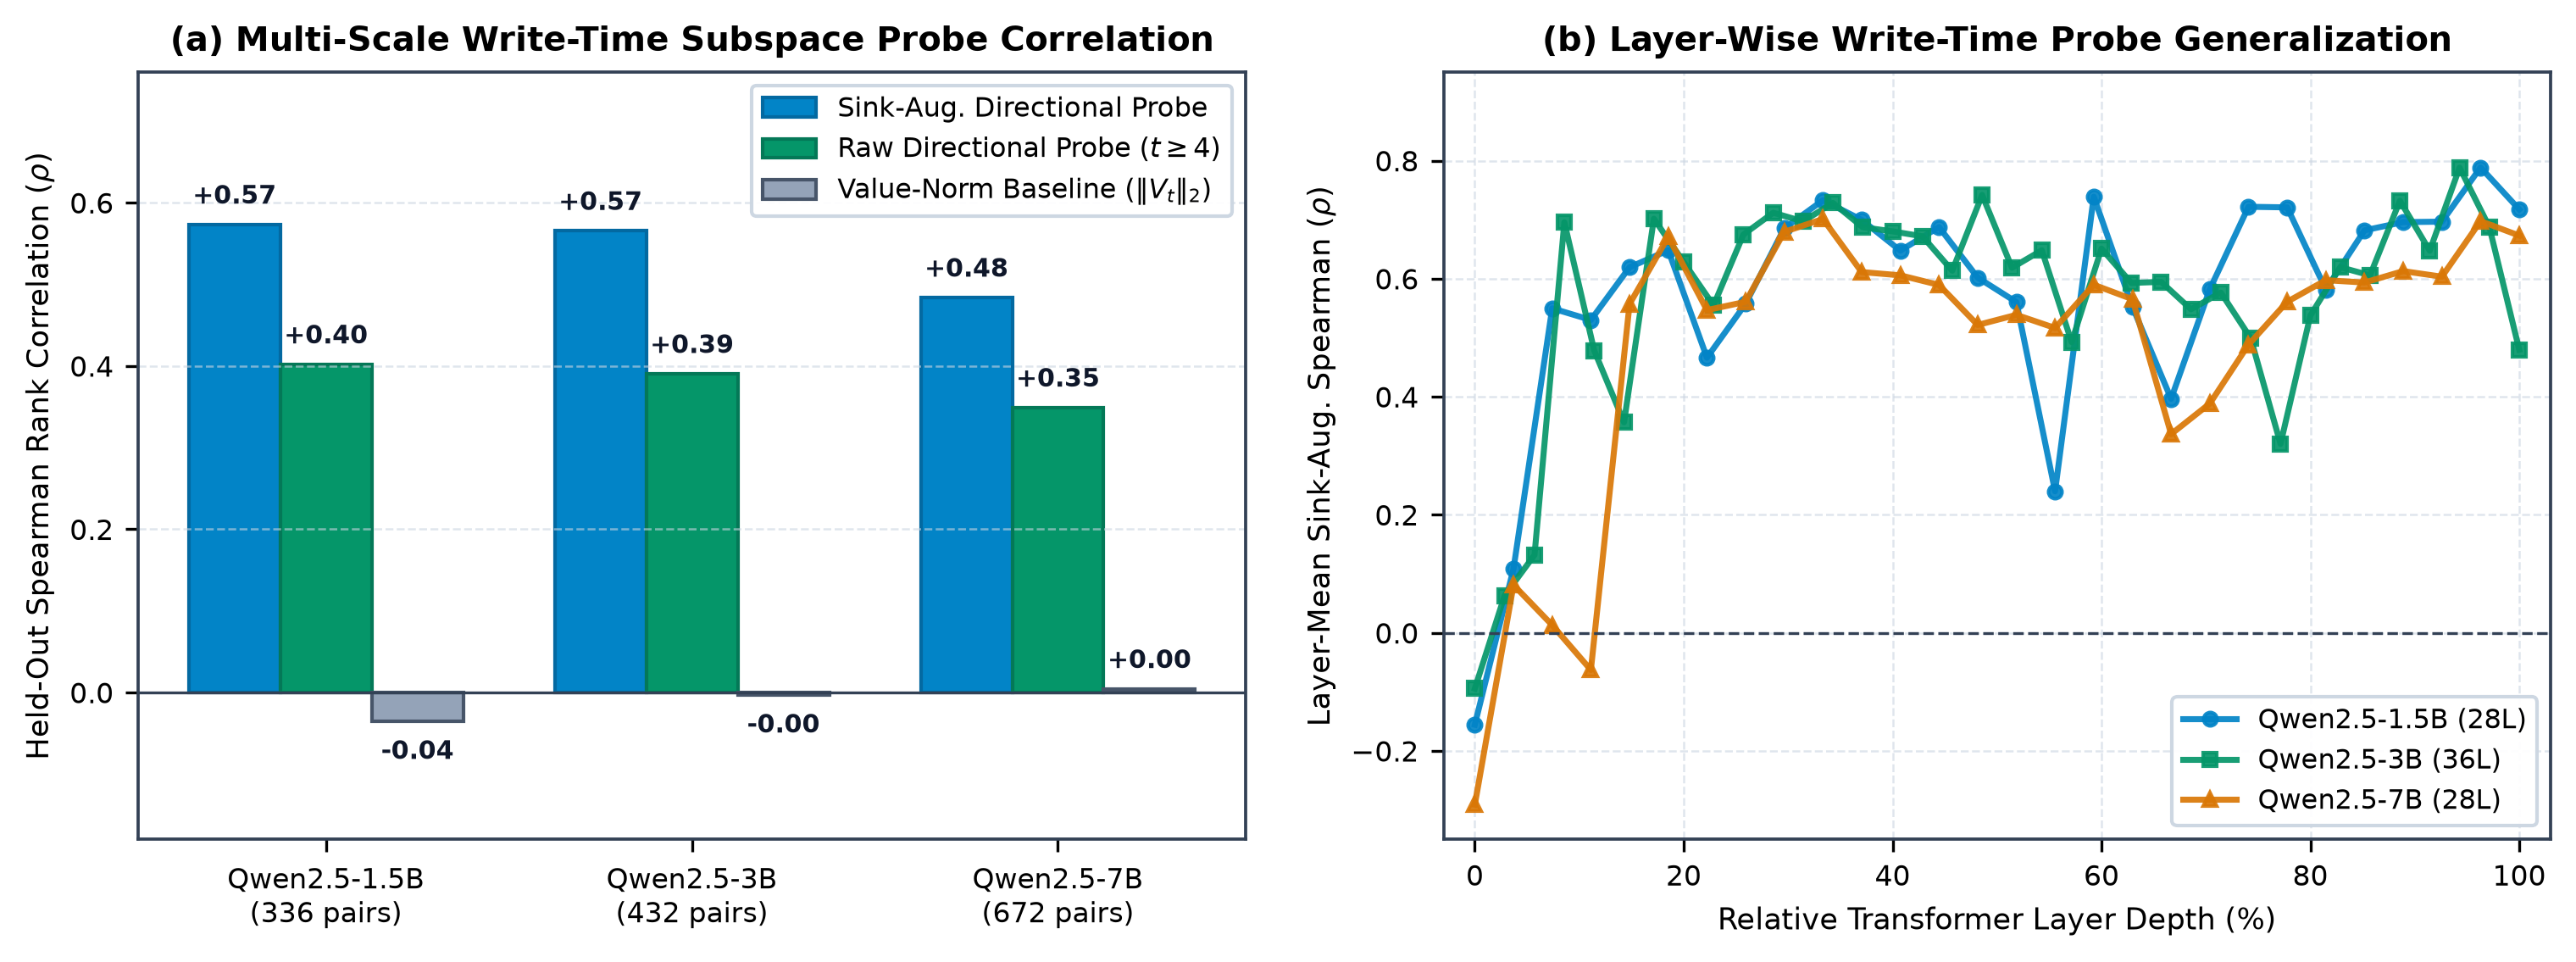
\includegraphics[width=\columnwidth]{probe_correlation.png}}
\caption{(a) Multi-scale held-out write-time probe Spearman $\rho$ across real pretrained \texttt{Qwen2.5-1.5B}, \texttt{3B}, and \texttt{7B} checkpoints versus $\|V_t\|_2$. (b) Layer-wise mean sink-augmented Spearman $\rho$ across relative transformer depth, showing strong generalization across middle and deep layers.}
\label{fig:probe_corr}
\end{figure}

\subsection{Multi-Scale Write-Time Probe and Distinct-Vector Codec Results}
Table~\ref{tab:probe_corr} and Fig.~\ref{fig:probe_corr} report write-time probe generalization across $1{,}440$ combined held-out (layer, prompt) pairs spanning \texttt{Qwen2.5-1.5B} ($336$ pairs), \texttt{3B} ($432$ pairs), and \texttt{7B} ($672$ pairs). Across all three scales, the value-norm baseline $\|V_t\|_2$ exhibits near-zero rank correlation ($\rho \in [-0.0354, +0.0043]$). Sign-aligned directional query-subspace probing lifts non-sink ($t \ge 4$) correlation to $\rho = 0.3491$--$0.4020$ and sink-augmented correlation to $\rho = 0.4838$--$0.5733$ ($49.72\%$--$52.64\%$ Recall@20\%). Notably, an earlier archived pre-sign-alignment prototype in our repository recorded negative probe correlation ($\rho = -0.0223$) and $0\%$ retrieval on 7B; adding sign-aligned uncentered eigendecomposition \eqref{eq:sign_align} and softplus gating \eqref{eq:write_probe_hf} directly resolved that failure mode.

\begin{table*}[t]
\caption{One-Step Ridge-Preconditioned Sparse Coding vs. OMP and 30-Step FISTA on 1,024 Strictly Distinct, Non-Tiled Real Paul Graham Prose KV Vectors (\texttt{Qwen2.5-1.5B} Layer 10, $d=128$, CUDA FP16)}
\begin{center}
\resizebox{\textwidth}{!}{%
\begin{tabular}{|c|c|c|c|c|c|c|c|c|c|c|c|}
\hline
\textbf{Sparsity} & \textbf{Payload} & \textbf{Ratio vs.} & \textbf{1-Step} & \textbf{OMP} & \textbf{FISTA} & \textbf{1-Step Enc.} & \textbf{1-Step Dec.} & \textbf{OMP Enc.} & \textbf{FISTA Enc.} & \textbf{Speedup} & \textbf{Speedup} \\
\textbf{$s$} & \textbf{(\texttt{3s+2})} & \textbf{FP16 (\texttt{256B})} & \textbf{Cosine} & \textbf{Cosine} & \textbf{Cosine} & \textbf{(ms)} & \textbf{(ms)} & \textbf{(ms)} & \textbf{(ms)} & \textbf{vs. OMP} & \textbf{vs. FISTA} \\
\hline
$s = 4$  & 14 B & $18.29\times$ & 0.4677 & 0.4736 & 0.4718 & \textbf{1.896} & 0.198 & 16.812 & 10.419 & \textbf{8.87$\times$}  & \textbf{5.50$\times$} \\
$s = 8$  & 26 B & $9.85\times$  & 0.5852 & 0.5921 & 0.5903 & \textbf{0.869} & 0.106 & 5.021  & 10.367 & \textbf{5.78$\times$}  & \textbf{11.93$\times$} \\
$s = 12$ & 38 B & $6.74\times$  & 0.6609 & 0.6686 & 0.6667 & \textbf{0.847} & 0.105 & 6.492  & 10.257 & \textbf{7.67$\times$}  & \textbf{12.11$\times$} \\
$s = 16$ & 50 B & $5.12\times$  & 0.7167 & 0.7249 & 0.7232 & \textbf{0.849} & 0.108 & 8.208  & 10.287 & \textbf{9.66$\times$}  & \textbf{12.11$\times$} \\
$s = 32$ & 98 B & $2.61\times$  & 0.8488 & 0.8586 & 0.8572 & \textbf{0.877} & 0.160 & 32.959 & 11.643 & \textbf{37.58$\times$} & \textbf{13.27$\times$} \\
\hline
\end{tabular}%
}
\label{tab:codec_results}
\end{center}
\end{table*}

\begin{figure}[t]
\centerline{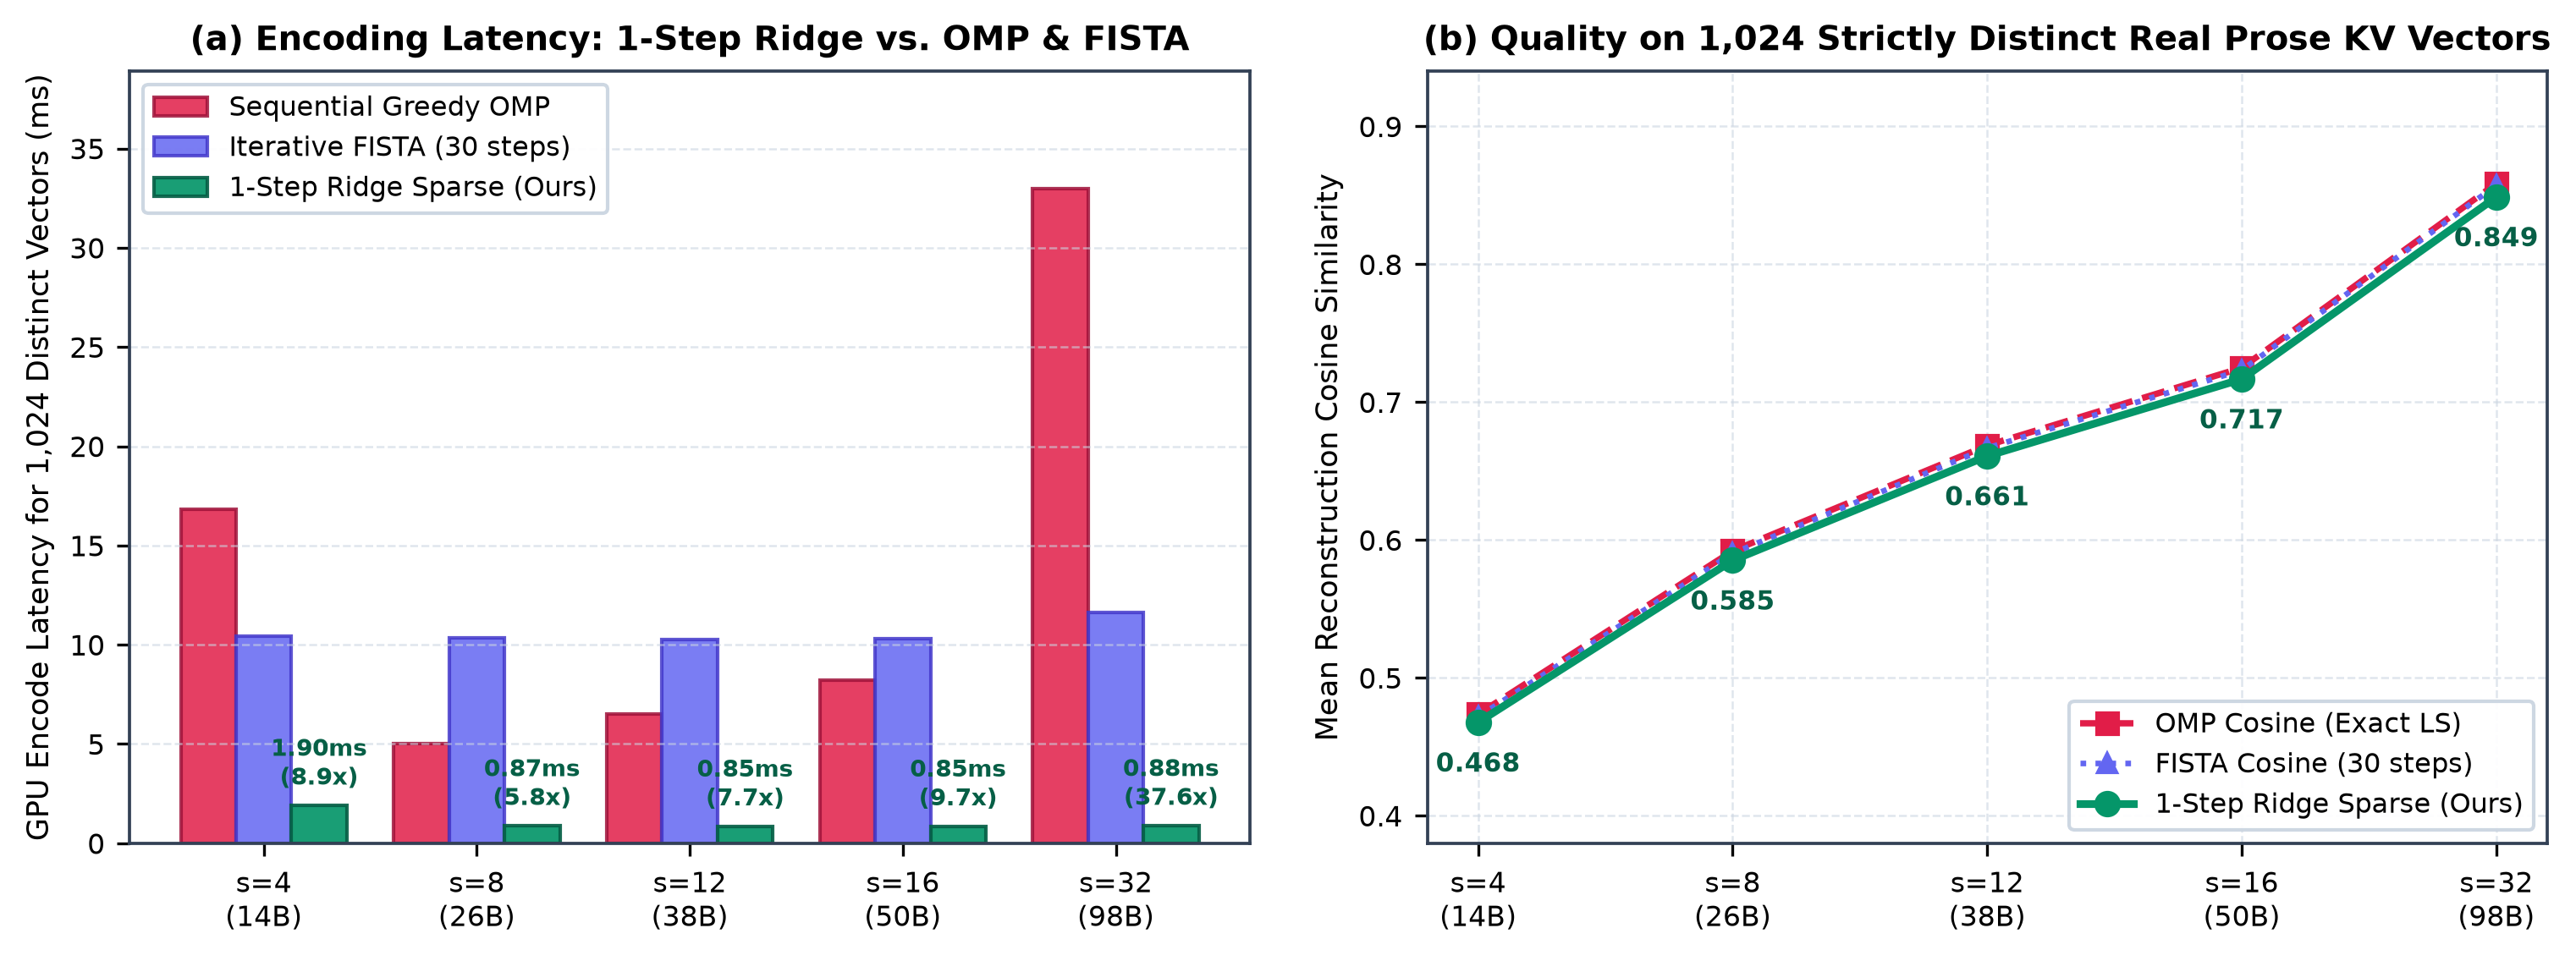
\includegraphics[width=\columnwidth]{elasticnet_vs_omp.png}}
\caption{GPU encoding latency and reconstruction cosine similarity of One-Step Ridge-Preconditioned Sparse Coding vs. OMP and 30-step FISTA on $1{,}024$ strictly distinct real Paul Graham prose KV vectors (\texttt{Qwen2.5-1.5B} layer 10).}
\label{fig:codec_bench}
\end{figure}

Table~\ref{tab:codec_results} and Fig.~\ref{fig:codec_bench} evaluate One-Step Ridge-Preconditioned Thresholded Sparse Coding on $1{,}024$ strictly distinct, non-tiled real prose KV vectors (avoiding any repeated-vector tiling). Across $s \in \{4, 8, 12, 16, 32\}$, our single-GEMM encoder stays within $0.0059$--$0.0098$ cosine similarity of exact iterative OMP while maintaining flat sub-millisecond steady-state latency ($0.847$--$0.877\text{ ms}$ for $s \ge 8$; $0.105$--$0.160\text{ ms}$ decode), delivering \textbf{$9.66\times$ speedup over OMP at $s=16$} and \textbf{$37.58\times$ at $s=32$} ($11.93\times$--$13.27\times$ over 30-step FISTA).

\subsection{External Paul Graham Essays NIAH Across 1.5B, 3B, and 7B}
Table~\ref{tab:pg_niah} and Fig.~\ref{fig:pareto} present our primary real-model retrieval benchmark on unseen 5-digit passkeys planted inside distinct external Paul Graham essays at an equalized $\sim 21\%$ KV budget (solved automatically via \texttt{solve\_equal\_budget\_params}). Every accuracy is reported with its exact numerator/denominator and $95\%$ Wilson confidence interval:
\begin{itemize}
    \item \textbf{Real \texttt{Qwen2.5-1.5B-Instruct} ($20$ unseen essays, $L \approx 1{,}024$):} \texttt{StoikovKV Hybrid} achieves \textbf{$17/20$ ($85.0\%$, $95\%$ CI $[64.0\%, 94.8\%]$)}---with $5/5$ at $10\%$ and $25\%$ depths---and the highest compressed next-token logit cosine ($0.9351$) at $21.56\%$ KV bytes ($22.26\%$ including shared dictionaries across only $3$ active layers). By comparison, \texttt{SnapKV} drops to $12/20$ ($60.0\%$, CI $[38.7\%, 78.1\%]$, cosine $0.7973$), \texttt{Standalone Lexico} drops to $5/20$ ($25.0\%$, $+27.56\%$ total memory with $28$-layer dictionaries, $4.70\text{ tok/s}$), and both \texttt{Standalone H2O} and \texttt{KIVI-2bit} score $0/20$ ($0.0\%$).
    \item \textbf{Real \texttt{Qwen2.5-3B-Instruct} ($16$ unseen essays, $L \approx 1{,}024$):} \texttt{StoikovKV Hybrid} achieves \textbf{$16/16$ ($100.0\%$, $95\%$ CI $[80.6\%, 100.0\%]$)} across all four depths at $20.65\%$ KV memory ($21.35\%$ with dictionaries) with $0.9371$ logit cosine ($3.06\times$ faster than \texttt{Standalone Lexico}'s $3.24\text{ tok/s}$). Notably, while \texttt{SnapKV} also hits $16/16$ on this single-turn essay format, its logit cosine collapses to $0.7161$ ($-0.2210$ below StoikovKV) because it discards global essay context outside the local suffix window, whereas \texttt{Standalone H2O} ($0/16$), \texttt{KIVI-2bit} ($1/16$), and \texttt{Standalone Lexico} ($5/16$) fail retrieval.
    \item \textbf{Real \texttt{Qwen2.5-7B-Instruct} ($8$ unseen essays, $L \approx 512$, GPU=7 / CPU=5 / NVMe=16 offloaded FP16):} \texttt{StoikovKV Hybrid} achieves \textbf{$8/8$ ($100.0\%$, $95\%$ CI $[67.6\%, 100.0\%]$)} across all four depths ($2/2$ each) at $20.75\%$ KV memory ($21.19\%$ including dictionaries across only $6/112$ Tier-2 heads) with \textbf{$0.8855$ next-token logit cosine}, outperforming \texttt{SnapKV} ($8/8$, cosine $0.7942$, $-0.0913$ lower fidelity) and \texttt{Standalone H2O} ($0/8$ [$0.0\%$], cosine $0.6985$). Throughput is NVMe/PCIe-offload bound at $0.24$--$0.25\text{ tok/s}$ across all policies on the $8\text{ GB}$ GPU; we emphasize that this 7B run validates exact unquantized FP16 retrieval quality and compression accounting rather than native GPU decode speed.
\end{itemize}

\begin{table*}[t]
\caption{External Kamradt Paul Graham Essays Needle-in-a-Haystack Evaluation Across Real Pretrained \texttt{Qwen2.5-1.5B}, \texttt{3B}, and \texttt{7B} Checkpoints (Strictly Unseen Passkeys $\neq \texttt{"94812"}$, Equalized $\sim 21\%$ KV Budget)}
\begin{center}
\resizebox{\textwidth}{!}{%
\begin{tabular}{|l|c|c|c|c|c|c|c|c|}
\hline
\textbf{Model / Policy} & \textbf{$\rho_{\text{keep}}$ / $s$} & \textbf{Hits / $N$} & \textbf{Acc. (\%)} & \textbf{Wilson 95\% CI} & \textbf{KV Mem \%} & \textbf{+Dict \%} & \textbf{Logit Cos.} & \textbf{Decode (tok/s)} \\
\hline
\multicolumn{9}{|c|}{\textit{Real \texttt{Qwen/Qwen2.5-1.5B-Instruct} (100\% GPU FP16, $N=20$ Essays, $L \approx 1{,}024$, Depths $\{10, 25, 50, 75\}\%$)}} \\
\hline
Full FP16          & 1.000 / 16 & 20 / 20 & 100.0\% & $[83.9, 100.0]\%$ & 100.00\% & 100.00\% & 1.0000 & 17.76 \\
Standalone H2O \cite{b2} & 0.193 / 16 & 0 / 20 & 0.0\% & $[0.0, 16.1]\%$ & 21.93\% & 21.93\% & 0.8912 & 14.89 \\
SnapKV \cite{b5}         & 0.193 / 16 & 12 / 20 & 60.0\% & $[38.7, 78.1]\%$ & 21.93\% & 21.93\% & 0.7973 & 16.28 \\
KIVI-2bit Quant \cite{b6}& 1.000 / 16 & 0 / 20 & 0.0\% & $[0.0, 16.1]\%$ & 19.89\% & 19.89\% & 0.5882 & 6.40 \\
Standalone Lexico \cite{b7}& 1.000 / 15 & 5 / 20 & 25.0\% & $[11.2, 46.9]\%$ & 21.03\% & 27.56\% & 0.8903 & 4.70 \\
\textbf{StoikovKV Hybrid} & \textbf{0.144 / 12} & \textbf{17 / 20} & \textbf{85.0\%} & \textbf{$[64.0, 94.8]\%$} & \textbf{21.56\%} & \textbf{22.26\%} & \textbf{0.9351} & \textbf{12.91} \\
\hline
\multicolumn{9}{|c|}{\textit{Real \texttt{Qwen/Qwen2.5-3B-Instruct} (100\% GPU FP16, $N=16$ Essays, $L \approx 1{,}024$, Depths $\{10, 25, 50, 75\}\%$)}} \\
\hline
Full FP16          & 1.000 / 16 & 16 / 16 & 100.0\% & $[80.6, 100.0]\%$ & 100.00\% & 100.00\% & 1.0000 & 13.98 \\
Standalone H2O \cite{b2} & 0.188 / 16 & 0 / 16 & 0.0\% & $[0.0, 19.4]\%$ & 21.84\% & 21.84\% & 0.7749 & 11.81 \\
SnapKV \cite{b5}         & 0.188 / 16 & 16 / 16 & 100.0\% & $[80.6, 100.0]\%$ & 21.84\% & 21.84\% & 0.7161 & 12.39 \\
KIVI-2bit Quant \cite{b6}& 1.000 / 16 & 1 / 16 & 6.2\% & $[1.1, 28.3]\%$ & 19.83\% & 19.83\% & 0.3159 & 4.93 \\
Standalone Lexico \cite{b7}& 1.000 / 15 & 5 / 16 & 31.2\% & $[14.2, 55.6]\%$ & 20.96\% & 27.33\% & 0.8441 & 3.24 \\
\textbf{StoikovKV Hybrid} & \textbf{0.132 / 11} & \textbf{16 / 16} & \textbf{100.0\%} & \textbf{$[80.6, 100.0]\%$} & \textbf{20.65\%} & \textbf{21.35\%} & \textbf{0.9371} & \textbf{9.92} \\
\hline
\multicolumn{9}{|c|}{\textit{Real \texttt{Qwen/Qwen2.5-7B-Instruct} (GPU=7 / CPU=5 / NVMe=16 Offloaded FP16, $N=8$ Essays, $L \approx 512$)}} \\
\hline
Full FP16          & 1.000 / 16 & 8 / 8 & 100.0\% & $[67.6, 100.0]\%$ & 100.00\% & 100.00\% & 1.0000 & 0.24 \\
Standalone H2O \cite{b2} & 0.158 / 16 & 0 / 8 & 0.0\% & $[0.0, 32.4]\%$ & 21.87\% & 21.87\% & 0.6985 & 0.24 \\
SnapKV \cite{b5}         & 0.158 / 16 & 8 / 8 & 100.0\% & $[67.6, 100.0]\%$ & 21.78\% & 21.78\% & 0.7942 & 0.24 \\
\textbf{StoikovKV Hybrid} & \textbf{0.106 / 9} & \textbf{8 / 8} & \textbf{100.0\%} & \textbf{$[67.6, 100.0]\%$} & \textbf{20.75\%} & \textbf{21.19\%} & \textbf{0.8855} & \textbf{0.25} \\
\hline
\end{tabular}%
}
\label{tab:pg_niah}
\end{center}
\end{table*}

\begin{figure}[t]
\centerline{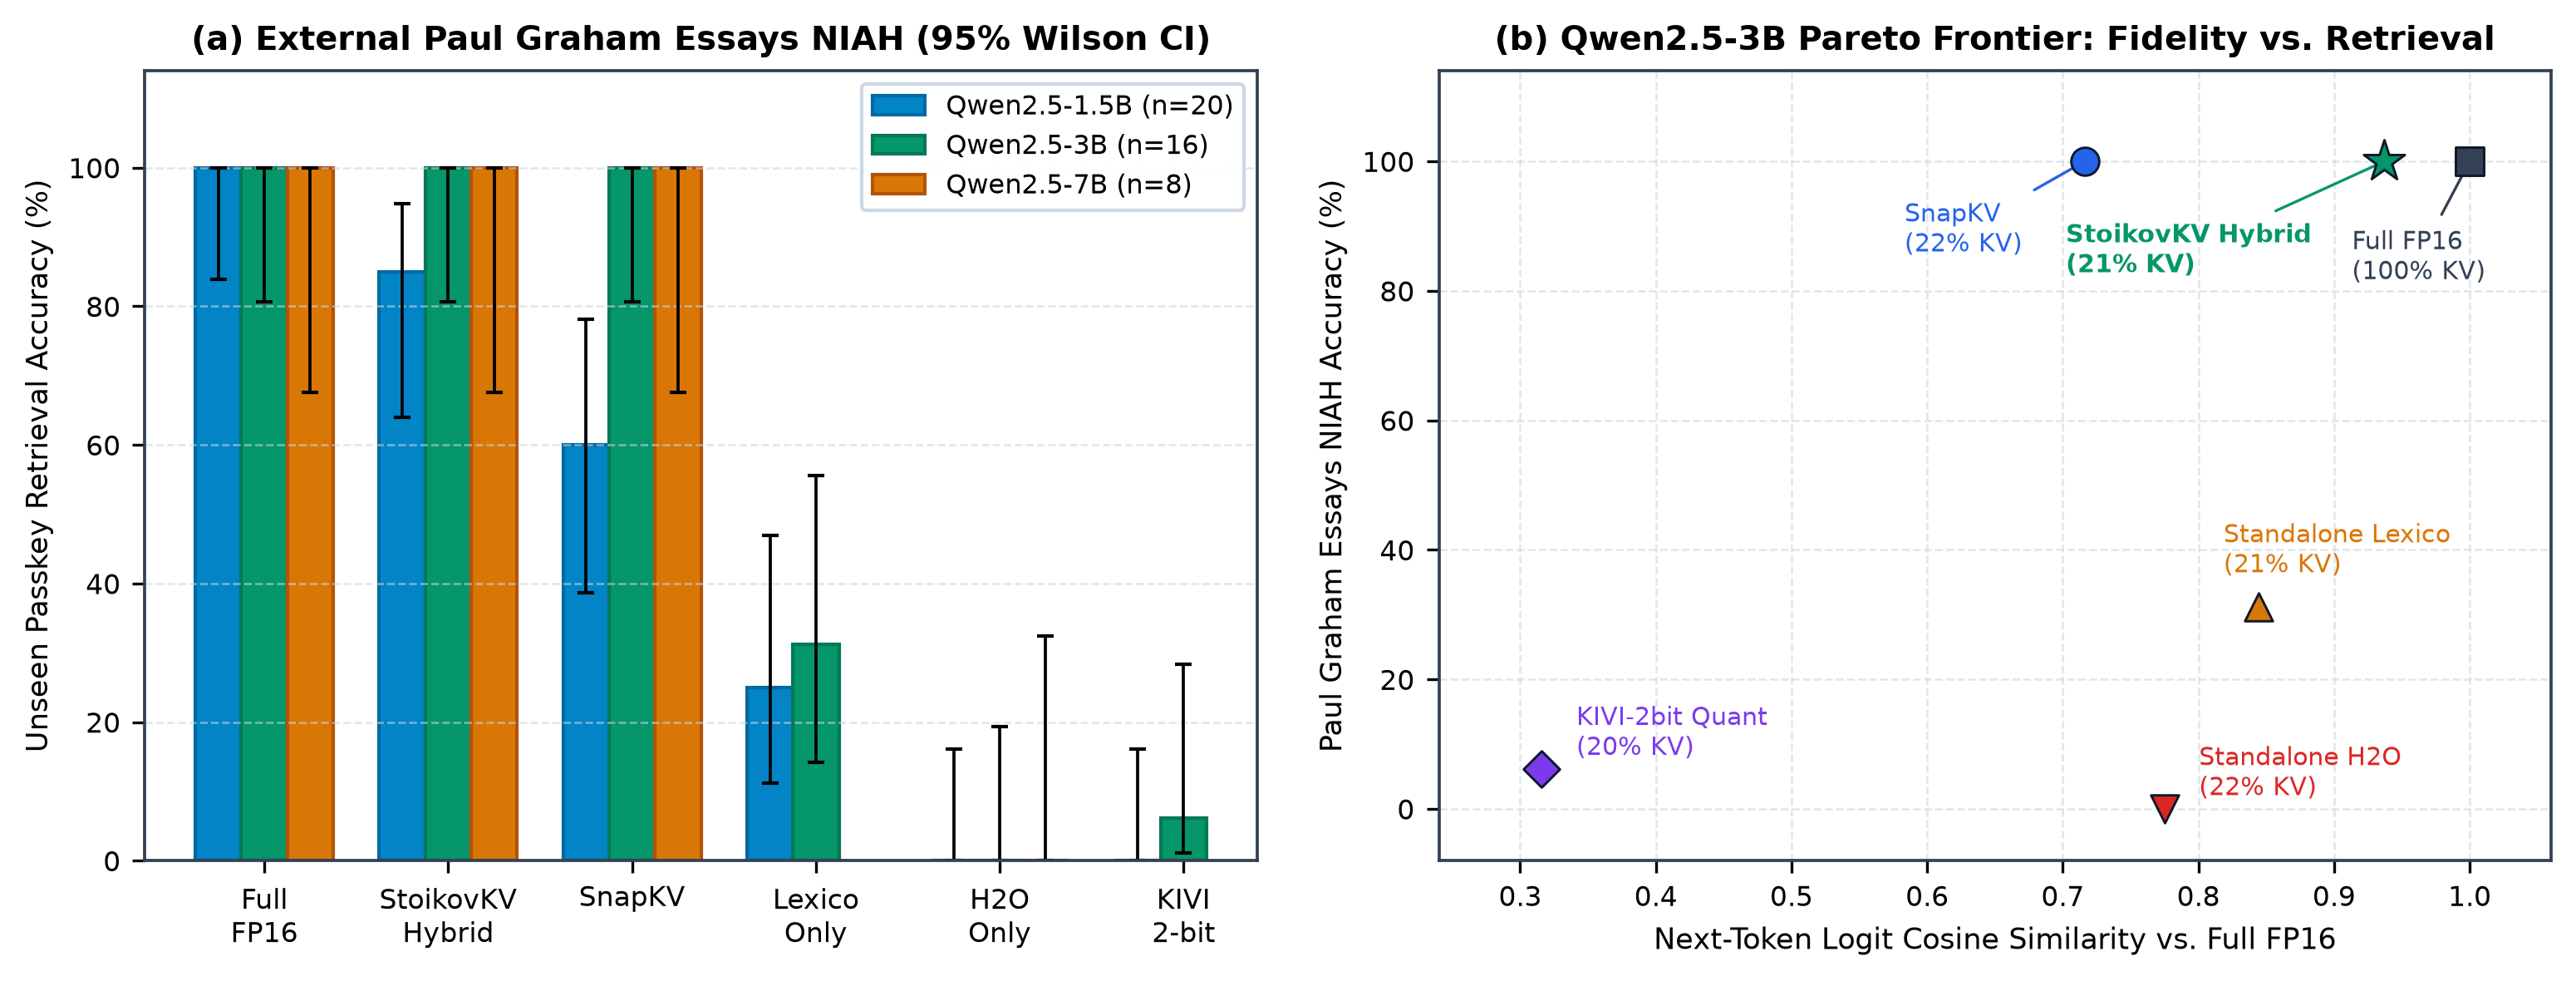
\includegraphics[width=\columnwidth]{pareto_quality_vs_bytes.png}}
\caption{(a) External Paul Graham Essays NIAH accuracy with exact $95\%$ Wilson confidence intervals across real \texttt{Qwen2.5-1.5B}, \texttt{3B}, and \texttt{7B} checkpoints. (b) Fidelity-vs-retrieval Pareto frontier on \texttt{Qwen2.5-3B}.}
\label{fig:pareto}
\end{figure}

\subsection{Multi-Turn Topic-Shift Ablation and Controlled GQA Suite}
To evaluate topic-shift adaptation specifically (where SnapKV's local observation window fails), Table~\ref{tab:multiturn} reports our controlled two-turn ablation on real \texttt{Qwen2.5-1.5B-Instruct} ($1{,}024$ tokens: Turn-1 systems notes with planted code across $4$ early depths $\{5\%, 12\%, 22\%, 35\%\}$, followed by an abrupt Turn-2 switch to CSS glassmorphism styling). Under this shift, \texttt{SnapKV} drops to $0/4$ ($0.0\%$, margin $-4.19$) and \texttt{Standalone H2O} retains $76.97\%$ stale Turn-1 slots ($23.03\%$ Turn-2 freshness, $3/4$ hits). By triggering $11$ online regime-change decay pulses, \texttt{StoikovKV Hybrid} lifts Turn-2 heavy-hitter freshness $2.94\times$ to \textbf{$67.70\%$}, achieves \textbf{$4/4$ ($100.0\%$, observed benchmark result)} with a $+7.63$ logit margin, and preserves $0.9850$ Turn-2 logit cosine at $20.56\%$ KV memory ($21.25\%$ with dictionaries)---running $2.16\times$ faster than \texttt{Standalone Lexico} ($3.09\text{ s}$ vs. $6.68\text{ s}$).

In our separate controlled standalone GQA harness (synthetic weights matching \texttt{Qwen2.5-1.5B} dimensions, $15$ runs $= 5\text{ trials} \times 3\text{ seeds}$ per cell across $L \in \{512, 2{,}048, 4{,}096\}$), \texttt{Standalone H2O} scores $0/15$ ($0\%$) on early ($10\%$) needles at every sequence length while \texttt{StoikovKV Hybrid} achieves $15/15$ across all $9$ length-depth cells ($135/135$). Similarly, on the compact $12$-layer/$4$-KV GQA WikiText-103 stream benchmark ($50$ passages), \texttt{StoikovKV Hybrid} sustains $1{,}910.8\text{ tok/s}$ ($2.78\times$ faster than \texttt{Standalone Lexico}'s $687.6\text{ tok/s}$) at $20.0\%$ KV memory with $15$ natural regime shifts; we emphasize that this throughput belongs to the compact standalone track rather than real 7B inference.

\begin{table}[t]
\caption{Controlled Two-Turn Topic-Shift Ablation on Real \texttt{Qwen2.5-1.5B-Instruct} ($L=1{,}024$, 4 Early Depths + Turn-2 CSS Shift)}
\begin{center}
\resizebox{\columnwidth}{!}{%
\begin{tabular}{|l|c|c|c|c|c|}
\hline
\textbf{Configuration} & \textbf{KV (+Dict)} & \textbf{Hits} & \textbf{Margin} & \textbf{CSS Cos.} & \textbf{T2 Fresh.} \\
\hline
Full FP16          & 100.0\% & 4/4 & $+7.09$ & 1.0000 & 40.04\% \\
Standalone H2O     & 21.9\%  & 3/4 & $+4.68$ & 0.9967 & 23.03\% \\
SnapKV             & 21.9\%  & 0/4 & $-4.19$ & 0.7703 & 37.92\% \\
KIVI-2bit Quant    & 19.9\%  & 0/4 & $-8.97$ & 0.0160 & 0.00\% \\
Standalone Lexico  & 21.0 (27.5)\% & 4/4 & $+3.99$ & 0.9621 & 0.00\% \\
\textbf{StoikovKV Hybrid} & \textbf{20.6 (21.3)\%} & \textbf{4/4} & \textbf{$+7.63$} & \textbf{0.9850} & \textbf{67.70\%} \\
\hline
\end{tabular}%
}
\label{tab:multiturn}
\end{center}
\end{table}

\subsection{Strict Lossless Speculative Parity and Memory-Ceiling Batch Scaling}
Table~\ref{tab:spec_audit} and Fig.~\ref{fig:matryoshka}(a) audit \texttt{matryoshka\_speculative\_generate} on real \texttt{Qwen2.5-1.5B-Instruct} with \texttt{strict\_rejection\_sampling=True} over $32$ generated tokens ($\gamma_{\text{spec}} = 4$, verify $s = 16$, unseen passkey \texttt{"62741"} in a Paul Graham essay). Under strict greedy verification (\texttt{do\_sample=False}), StoikovKV achieves \textbf{$32/32$ ($100.0\%$) bit-exact token parity} against sequential $s=16$ target decoding across every draft sparsity $m \in \{2, 4, 8, 12\}$ ($\alpha = 1.0000$, $4.71\text{ tok/cycle}$, $65.90\%$--$66.34\%$ KV read bandwidth saved vs. Full FP16). Under strict stochastic Leviathan rejection sampling ($T = 0.7$, \texttt{top\_k=32}, seed $42$), empirical acceptance reaches $\alpha = 0.9259$ at $m=2$ ($E[\alpha] = 0.9574$) and $\alpha = 0.9630$ for $m \in \{4, 8, 12\}$ ($E[\alpha] = 0.9735$--$0.9908$, $4.71\text{ tok/cycle}$).

\begin{table}[t]
\caption{Strict Lossless Matryoshka Speculative Audit (\texttt{strict\_rejection\_sampling=True}, Real \texttt{Qwen2.5-1.5B}, $\gamma=4, s=16$)}
\begin{center}
\resizebox{\columnwidth}{!}{%
\begin{tabular}{|c|c|c|c|c|c|}
\hline
\textbf{Draft} & \textbf{Greedy} & \textbf{Greedy} & \textbf{Stoch. ($T{=}0.7$)} & \textbf{Stoch.} & \textbf{BW Saved} \\
\textbf{$m$ (Bytes)} & \textbf{Exact Parity} & \textbf{$\alpha$ / tok/cyc} & \textbf{Emp. $\alpha$ ($E[\alpha]$)} & \textbf{tok/cyc} & \textbf{vs. FP16} \\
\hline
$m=2$ (8 B)  & \textbf{32/32 (100\%)} & 1.00 / 4.71 & 0.9259 (0.9574) & 4.12 & \textbf{66.34\%} \\
$m=4$ (14 B) & \textbf{32/32 (100\%)} & 1.00 / 4.71 & 0.9630 (0.9735) & 4.71 & \textbf{66.25\%} \\
$m=8$ (26 B) & \textbf{32/32 (100\%)} & 1.00 / 4.71 & 0.9630 (0.9856) & 4.71 & 66.07\% \\
$m=12$ (38 B)& \textbf{32/32 (100\%)} & 1.00 / 4.71 & 0.9630 (0.9908) & 4.71 & 65.90\% \\
\hline
\end{tabular}%
}
\label{tab:spec_audit}
\end{center}
\end{table}

\begin{figure}[t]
\centerline{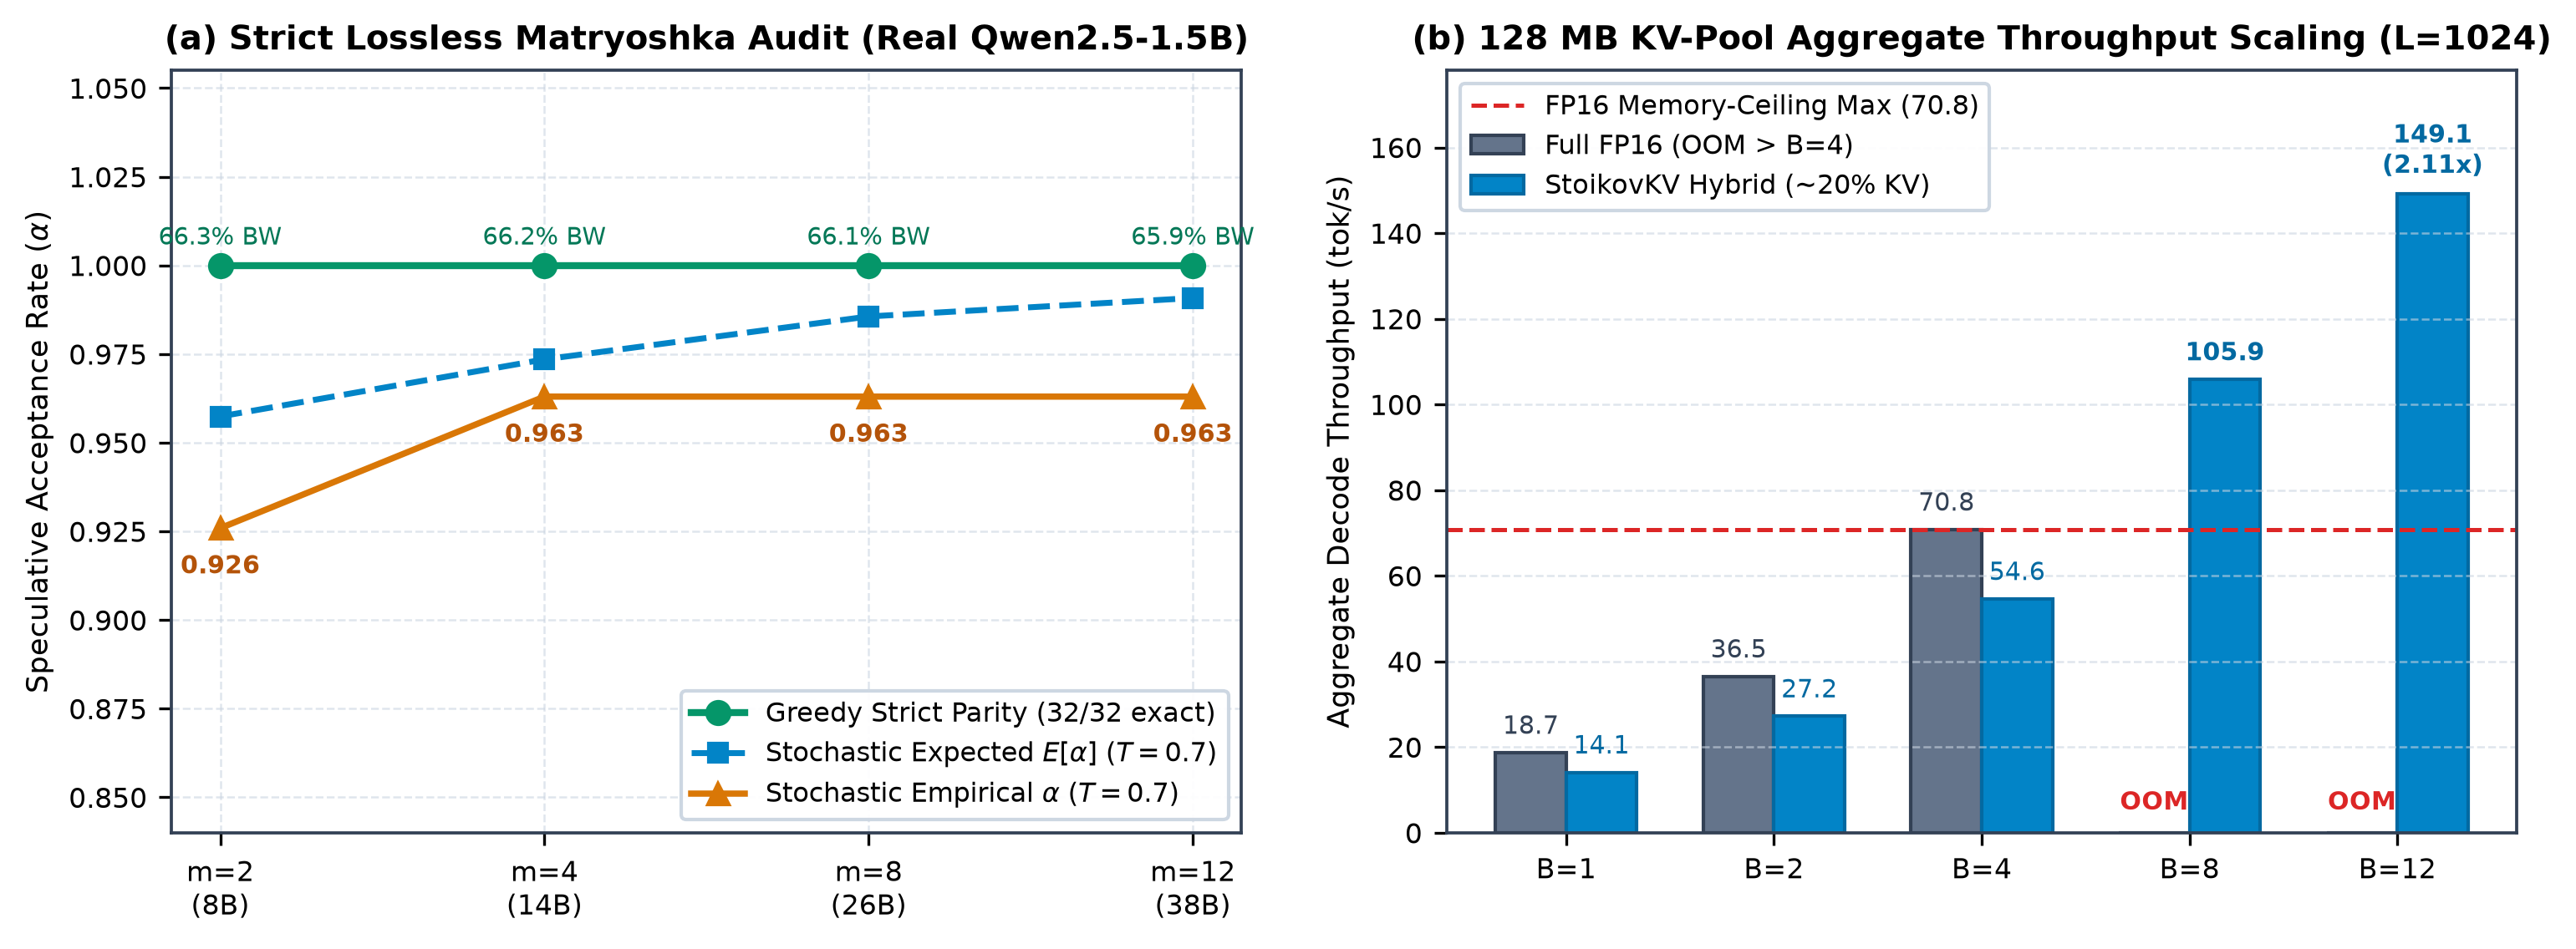
\includegraphics[width=\columnwidth]{matryoshka_acceptance.png}}
\caption{(a) Strict lossless Matryoshka speculative acceptance on real \texttt{Qwen2.5-1.5B-Instruct} ($32/32$ greedy parity; $T=0.7$ rejection sampling). (b) Aggregate decode throughput under an imposed $128\text{ MB}$ KV-pool cap ($L=1{,}024$).}
\label{fig:matryoshka}
\end{figure}

Finally, Table~\ref{tab:batch_scaling} and Fig.~\ref{fig:matryoshka}(b) evaluate multi-batch memory-ceiling scalability on real \texttt{Qwen2.5-1.5B-Instruct} under an imposed \textbf{$128\text{ MB}$ KV-cache pool cap} (excluding model weights and activation buffers) using replicated $L = 1{,}024$ prompts, timing strictly $16$ CUDA-synchronized autoregressive decode steps (prefill excluded). At matched batch sizes ($B \in \{1, 2, 4\}$), Python-level per-head routing makes StoikovKV $\sim 23\%$--$25\%$ slower than raw FP16 ($54.6$ vs. $70.8\text{ tok/s}$ at $B=4$). However, because \texttt{Full FP16} consumes $27.48\text{ MB/request}$ and exhausts the $128\text{ MB}$ KV pool above $B=4$ ($109.92\text{ MB}$, peaking at $70.8\text{ tok/s}$), whereas \texttt{StoikovKV Hybrid} physically compacts the per-request KV footprint by $4.56\times$ to $6.03\text{ MB}$, StoikovKV scales cleanly to $B=8$ ($48.22\text{ MB}$, $105.9\text{ tok/s}$) and $B=12$ ($72.33\text{ MB}$, \textbf{$149.1\text{ tok/s}$})---a \textbf{$2.11\times$ higher maximum aggregate throughput under the $128\text{ MB}$ KV-pool constraint} (not an intrinsic per-request decode speedup).

\begin{table}[t]
\caption{Memory-Ceiling Aggregate Decode Throughput on Real \texttt{Qwen2.5-1.5B-Instruct} (Imposed $128\text{ MB}$ KV Pool, $L=1{,}024$, 16 Synchronized Decode Steps)}
\begin{center}
\resizebox{\columnwidth}{!}{%
\begin{tabular}{|c|c|c|c|c|}
\hline
\textbf{Batch} & \multicolumn{2}{c|}{\textbf{Full FP16 KV Cache}} & \multicolumn{2}{c|}{\textbf{StoikovKV Hybrid ($\sim$20\%)}} \\
\cline{2-5}
\textbf{Size $B$} & \textbf{Phys. KV} & \textbf{Agg. tok/s} & \textbf{Phys. KV} & \textbf{Agg. tok/s} \\
\hline
$B = 1$  & 27.48 MB  & 18.7 & \textbf{6.03 MB}  & 14.1 \\
$B = 2$  & 54.96 MB  & 36.5 & \textbf{12.05 MB} & 27.2 \\
$B = 4$  & 109.92 MB & \textbf{70.8 (Cap)} & \textbf{24.11 MB} & 54.6 \\
$B = 8$  & 227.50 MB & \textit{Pool OOM} & \textbf{48.22 MB} & \textbf{105.9} \\
$B = 12$ & 341.25 MB & \textit{Pool OOM} & \textbf{72.33 MB} & \textbf{149.1 (2.11$\times$)} \\
\hline
\end{tabular}%
}
\label{tab:batch_scaling}
\end{center}
\end{table}

\section{Limitations and Discussion}
We highlight four current limitations that frame future engineering work:
\begin{enumerate}
    \item \textbf{Single-Request Python Dispatch Overhead:} At small batch sizes ($B \le 4$) where the full FP16 KV cache already fits in GPU memory, PyTorch-level per-head slicing and dictionary gather operations incur $\sim 23\%$--$25\%$ latency overhead compared to contiguous FP16 SDPA. Fusing Tier-1 compaction and Tier-2 sparse reconstruction into custom Triton/CUDA kernels is needed to realize wall-clock single-request speedups in addition to memory-ceiling concurrency gains.
    \item \textbf{Hardware Offloading on 7B+ Models:} Because our evaluation hardware is an $8\text{ GB}$ VRAM RTX 4060 Laptop with $15\text{ GB}$ host RAM, exact FP16 evaluation of \texttt{Qwen2.5-7B-Instruct} ($14.8\text{ GB}$ weights) requires GPU/CPU/NVMe layer offloading. While this validates exact unquantized FP16 probe correlation, head routing, and NIAH retrieval quality, absolute 7B wall-clock throughput is bound by PCIe/NVMe streaming rather than HBM bandwidth; native GPU throughput benchmarking at 7B--70B scale on multi-GPU or $24$--$80\text{ GB}$ accelerators remains future work.
    \item \textbf{One-Step Approximation Gap and Dictionary Amortization:} Our one-step preconditioned sparse encoder trails exact OMP by $0.006$--$0.010$ cosine similarity and carries $64\text{ KB}$ of static $(D_l, W_{\text{ridge},l})$ overhead per active Tier-2 layer, which amortizes only beyond $L^* \approx 318$ vectors per layer (and is minimized by co-locating Tier-2 heads onto $\sim 11\%$ of layers).
    \item \textbf{Calibration Domain Shift:} Although retrieval-head identity transfers strongly from $4$ synthetic calibration prompts to unseen Paul Graham essays, extreme modality or language shifts (e.g., dense source code or non-Latin scripts) can degrade static dictionary reconstruction, motivating periodic online Sherman--Morrison rank-1 updates of $(D_l, W_{\text{ridge},l})$.
\end{enumerate}

\section{Conclusion}
We presented StoikovKV, a heterogeneous per-KV-head compression and self-speculative decoding engine for GQA language models. By separating one-time streaming hook calibration from strictly FlashAttention-compatible online inference, combining sign-aligned write-time query-subspace probing with three-tier head routing, online regime-change heavy-hitter decay, One-Step Ridge-Preconditioned Thresholded Sparse Coding, and strict lossless Matryoshka speculative verification, StoikovKV preserves long-range passkey retrieval and next-token logit fidelity across real \texttt{Qwen2.5-1.5B}, \texttt{3B}, and \texttt{7B} checkpoints at $\sim 21\%$ KV memory while expanding memory-capped batch serving throughput by $2.11\times$.

\section*{Code, Data, and Reproducibility}
The complete StoikovKV source code, all $20/20$ automated unit tests, reproducible audit scripts (\texttt{benchmarks/bench\_real\_models\_audit.py}), and a SHA-256 provenance manifest (\texttt{benchmarks/results/experiment\_manifest.json}) pinning exact Git commits, source hashes, and HuggingFace model revisions (\texttt{Qwen2.5-1.5B}: \texttt{989aa79}, \texttt{3B}: \texttt{aa8e725}, \texttt{7B}: \texttt{a09a354}) are publicly available at \url{https://github.com/sairishigangarapu/StoikovKV}. External evaluations use the public Kamradt Paul Graham Essays NIAH corpus \cite{b15} and WikiText-103 \cite{b16}.

\begin{thebibliography}{00}
\bibitem{b1} J. Ainslie, J. Lee-Thorp, M. de Jong, Y. Zemlyanskiy, F. Lebr\'{o}n, and S. Sanghai, ``GQA: Training generalized multi-query transformer models from multi-head checkpoints,'' in \textit{Proc. Conf. Empirical Methods Natural Lang. Process. (EMNLP)}, 2023, pp. 4895--4901.
\bibitem{b2} Z. Zhang, Y. Sheng, T. Zhou, T. Chen, L. Zheng, R. Cai, Z. Song, Y. Tian, C. R\'{e}, C. Barrett, Z. Wang, and B. Chen, ``H2O: Heavy-hitter oracle for efficient generative inference of large language models,'' in \textit{Adv. Neural Inf. Process. Syst. (NeurIPS)}, vol. 36, 2023, pp. 34661--34710.
\bibitem{b3} G. Xiao, Y. Tian, B. Chen, S. Han, and M. Lewis, ``Efficient streaming language models with attention sinks,'' in \textit{Proc. Int. Conf. Learn. Represent. (ICLR)}, 2024.
\bibitem{b4} T. Dao, ``FlashAttention-2: Faster attention with better parallelism and work partitioning,'' in \textit{Proc. Int. Conf. Learn. Represent. (ICLR)}, 2024.
\bibitem{b5} Y. Li, Y. Huang, B. Yang, B. Venkitesh, A. Locatelli, H. Ye, T. Cai, P. Lewis, and D. Chen, ``SnapKV: LLM knows what you are looking for before generation,'' in \textit{Adv. Neural Inf. Process. Syst. (NeurIPS)}, vol. 37, 2024.
\bibitem{b6} Z. Liu, J. Yuan, H. Jin, S. Zhong, Z. Xu, V. Braverman, B. Chen, and X. Hu, ``KIVI: A tuning-free asymmetric 2bit quantization for KV cache,'' in \textit{Proc. Int. Conf. Mach. Learn. (ICML)}, 2024.
\bibitem{b7} J. Kim, J. Park, J. Cho, and D. Papailiopoulos, ``Lexico: Extreme KV cache compression via sparse coding over universal dictionaries,'' in \textit{Proc. Int. Conf. Mach. Learn. (ICML)}, 2025 (arXiv:2412.08890).
\bibitem{b8} A. Beck and M. Teboulle, ``A fast iterative shrinkage-thresholding algorithm for linear inverse problems,'' \textit{SIAM J. Imag. Sci.}, vol. 2, no. 1, pp. 183--202, 2009.
\bibitem{b9} J. Su, M. Ahmed, Y. Lu, S. Pan, W. Bo, and Y. Liu, ``RoFormer: Enhanced transformer with rotary position embedding,'' \textit{Neurocomputing}, vol. 568, p. 127063, 2024.
\bibitem{b10} A. Kusupati, G. Bhatt, A. Rege, M. Wallingford, A. Sinha, V. Ramanujan, W. Howard-Snyder, K. Chen, S. Kakade, P. Jain, and A. Farhadi, ``Matryoshka representation learning,'' in \textit{Adv. Neural Inf. Process. Syst. (NeurIPS)}, vol. 35, 2022, pp. 30233--30249.
\bibitem{b11} A. Yang, B. Yang, B. Zhang, B. Hui, B. Zheng, B. Yu, C. Li, D. Liu, F. Huang, H. Wei, H. Lin, J. Yang, J. Tu, J. Zhang, J. Yang, J. Yang, J. Zhou, and J. Lin, ``Qwen2.5 technical report,'' \textit{arXiv preprint arXiv:2412.15115}, 2024.
\bibitem{b12} Y. Leviathan, M. Kalman, and Y. Matias, ``Fast inference from transformers via speculative decoding,'' in \textit{Proc. Int. Conf. Mach. Learn. (ICML)}, 2023, pp. 19274--19286.
\bibitem{b13} M. Avellaneda and S. Stoikov, ``High-frequency trading in a limit order book,'' \textit{Quantitative Finance}, vol. 8, no. 3, pp. 217--224, Apr. 2008.
\bibitem{b14} W. Wu, Y. Wang, G. Xiao, H. Peng, and Y. Fu, ``Retrieval head mechanistically explains long-context factuality,'' in \textit{Proc. Int. Conf. Learn. Represent. (ICLR)}, 2025 (arXiv:2404.15574).
\bibitem{b15} G. Kamradt, ``LLMTest\_NeedleInAHaystack: Pressure testing LLMs,'' GitHub repository, 2023. [Online]. Available: \url{https://github.com/gkamradt/LLMTest_NeedleInAHaystack}
\bibitem{b16} S. Merity, C. Xiong, J. Bradbury, and R. Socher, ``Pointer sentinel mixture models,'' in \textit{Proc. Int. Conf. Learn. Represent. (ICLR)}, 2017.
\end{thebibliography}

\end{document}
